%Dokumentklasse
\documentclass[a4paper,12pt,oneside,pointlessnumbers]{scrbook}
\usepackage[left= 2.5cm,right = 2cm, bottom = 4 cm]{geometry}
%\usepackage[onehalfspacing]{setspace}
% ============= Packages =============

% Dokumentinformationen
\usepackage[
	pdftitle={Dokumentation},
	pdfsubject={},
	pdfauthor={Michael Stroh, Daniel Schwenk},
	pdfkeywords={},	
	%Links nicht einrahmen
	hidelinks
]{hyperref}


% Standard Packages
\usepackage[utf8]{inputenc}
\usepackage[ngerman]{babel}
\usepackage[T1]{fontenc}
\usepackage{graphicx, subfig}
\graphicspath{{img/}}
\usepackage{fancyhdr}
\usepackage{lmodern}
\usepackage{color}
\usepackage{pdfpages} 
\usepackage{listings}
\usepackage{adjustbox}
\usepackage{multirow}
%\usepackage[printonlyused]{acronym}
\usepackage{acronym}
\usepackage[nomain,acronym,xindy,toc]{glossaries}

% zusätzliche Schriftzeichen der American Mathematical Society
\usepackage{amsfonts}
\usepackage{amsmath}


%nicht einrücken nach Absatz
\setlength{\parindent}{0pt}


% ============= Kopf- und Fußzeile =============
\pagestyle{fancy}
%
\lhead{}
\chead{}
\rhead{\slshape \leftmark}
%%
\lfoot{}
\cfoot{\thepage}
\rfoot{}
%%
\renewcommand{\headrulewidth}{0.4pt}

\renewcommand{\footrulewidth}{0pt}

% ============= Package Einstellungen & Sonstiges ============= 
%Besondere Trennungen
\hyphenation{De-zi-mal-tren-nung}


% ============= Listing Style Definitionen ============= 

\lstdefinestyle{customc}{
  belowcaptionskip=1\baselineskip,
  breaklines=true,
  frame=L,
  xleftmargin=\parindent,
  language=C,
  showstringspaces=false,
  basicstyle=\footnotesize\ttfamily,
  %keywordstyle=\bfseries\color{green!40!black},
  %commentstyle=\itshape\color{purple!40!black},
  %identifierstyle=\color{blue},
  %stringstyle=\color{orange},
}

\lstdefinestyle{customasm}{
  belowcaptionskip=1\baselineskip,
  frame=L,
  xleftmargin=\parindent,
  language=[x86masm]Assembler,
  basicstyle=\footnotesize\ttfamily,
  %commentstyle=\itshape\color{purple!40!black},
}

\lstdefinestyle{customccolor}{
  belowcaptionskip=1\baselineskip,
  breaklines=true,
  frame=L,
  xleftmargin=\parindent,
  language=C,
  showstringspaces=false,
  basicstyle=\ttfamily,
  keywordstyle=\color{blue}\ttfamily,
  stringstyle=\color{red}\ttfamily,
  commentstyle=\color{green}\ttfamily,
  morecomment=[l][\color{magenta}]{\#}
}

\lstset{aboveskip=15pt,belowskip=15pt}


% ============= Dokumentbeginn =============

\begin{document}
%Seiten ohne Kopf- und Fußzeile sowie Seitenzahl
\pagestyle{empty}



\begin{figure}%
    \centering
    \subfloat{{
\includegraphics[scale=0.35]{img/hs_weingarten.png} }}%
    \qquad \qquad \qquad \qquad \qquad \qquad
    \subfloat{{
\includegraphics[scale=0.22]{img/ai.jpg} }}%
\end{figure}


\begin{center}
\begin{tabular}{p{\textwidth}}

\\

\begin{center}
\LARGE{\textsc{
Dokumentation \\
}}
\end{center}

\\


\begin{center}
\large{zur Vorlesung Systemadministration \\
im Bachelor Studiengang Angewandte Informatik \\}
\end{center}

\\

\begin{center}
\large{Wintersemester 2016 / 2017 \\
 bei Herrn Prof. Dr. rer. nat. Eggendorfer\\}
\end{center}

\\


\begin{center}
\huge{\textbf{Umsetzung eines Honeypots}} \\
\end{center}


\\

\\


\begin{center}
\large{\textbf{Michael Stroh}} \\
\small{Matrikelnr. 24972}
\end{center}

\begin{center}
\large{\textbf{Daniel Schwenk}} \\
\small{Matrikelnr. 24961}

\end{center}

\\

\\

\begin{center}
\large{02. Dezember 2016}
\end{center}




\end{tabular}
\end{center}

% Beendet eine Seite und erzwingt auf den nachfolgenden Seiten die Ausgabe aller Gleitobjekte (z.B. Abbildungen), die bislang definiert, aber noch nicht ausgegeben wurden. Dieser Befehl fügt, falls nötig, eine leere Seite ein, sodaß die nächste Seite nach den Gleitobjekten eine ungerade Seitennummer hat. 
\cleardoubleoddpage

\pagestyle{fancy}

\pagenumbering{roman} % römische nummerieung für Abbildungsverzeichnis + Tabellenverzeichnis


%Inhaltsverzeichnis
\tableofcontents

%\newpage % new page, damit nummerierung passt ...
% Abbküzrungsverzeichnis in Inhaltsverzeichnis aufnehmen
\addcontentsline{toc}{chapter}{Abbkürzungsverzeichnis}
\chapter*{Abkürzungsverzeichnis}

\begin{acronym}[extNTFSaaa]
 \acro{DNS}{Domain Name System}
 \acro{FTP}{File Transfer Protocol}
 \acro{HIHP}{high-interaction honeypot}
 \acro{HTTP}{Hypertext Transfer Protocol} 
 \acro{LIHP}{low-interaction honeypot}
 \acro{LTS}{Long Term Support}
 \acro{MIHP}{mediium-interaction honeypot}
 \acro{SSH}{Secure Shell} 
 \acro{SQL}{Structured Query Language}

\end{acronym}

%\newpage % new page, damit nummerierung passt ...
% Abbildungsverzeichnis in Inhaltsverzeichnis aufnehmen
%\addcontentsline{toc}{chapter}{Abbildungsverzeichnis}
%Verzeichnis aller Bilder
%\listoffigures

%\newpage % new page, damit nummerierung passt ...
% Tabellenverzeichnis in Inhaltsverzeichnis aufnehmen
%\addcontentsline{toc}{chapter}{Tabellverzeichnis}
%Verzeichnis aller Tabellen
%\listoftables


% pagestyle für gesamtes Dokument aktivieren
\pagestyle{fancy}

\pagenumbering{arabic}
\chapter{Einleitung}
\label{ch:einleitung}

Das Internet und die Digitalisierung, die in alle Lebensbereiche Einzug hält, verändern Gesellschaft, Wirtschaft und Kultur. Egal ob im privaten oder beruflichen Umfeld, egal ob Arbeitsplatz-Computer, Smartphone oder Embedded System ständig sind wir von Computern umgeben. Die Verbreitung sowie die Vernetzung dieser Geräte untereinander wird in den nächsten Jahren im Zuge der "`Internet-der-Dinge-Evolution"' weiter drastisch zunehmen.\\


Ein oft vernachlässigter Aspekt ist hierbei das Thema "`IT-Sicherheit"'. Keine Software ist frei von Fehlern und Sicherheitslücken. Falsch konfigurierte Dienste und Software, die nicht regelmäßig aktualisiert wird, sind ein leichtes Ziel für Angreifer. Durch die zunehmende Vernetzung wird das Thema IT-Sicherheit in Zukunft weiter an Bedeutung gewinnen.\\

Um eine Infrastruktur, egal ob im privaten oder geschäftlichen Bereich, vor möglichen Angriffen zu schützen bedarf es eines immer größeren Aufwandes.



\section{Motivation}
\label{sec:Motivation}

Die Gewährleistung der IT-Sicherheit ist mittlerweile eine immens wichtige, wenn nicht sogar die wichtigste Anforderung an eine intakte IT-Infrastruktur. Entsprechend sollte ein Systemadministrator über ein breites Spektrum an Wissen im Bereich der IT-Sicherheit besitzen sowie in der Lage sein, mögliche Angriffsszenarien frühzeitig zu erkennen.\\


Das Konzept eines Honeypots, also einen potentiellen Angreifer nicht nur vor eigentlich wichtigen System fernzuhalten, sondern auch noch von seinem Wissen zu profitieren, stellt dabei einen hochspannenden Ansatz dar. 
Dieser Ansatz soll dem Projektteam helfen, Wissen über mögliche Angriffsszenarien und Vorgehensweisen zu erlangen, um so die Sicherheit von bestehenden und zukünftigen Infrastrukturen gewährleisten zu können.

\newpage


\section{Ziele}
\label{sec:Ziele}

Ziel dieser Arbeit ist es, ein System zu entwickeln, das als Honeypot dient. Dieser Honeypot soll eingesetzt werden, um Einblicke in die Vorgehensweise eines Angreifers zu bekommen. 
Das System stellt dazu ein vermeintlich leicht angreifbaren Webserver sowie SSH-Server dar.\\


Jegliche Zugriffe und Aktivitäten die ein Angriff hinterlässt werden protokolliert und ausgewertet. Das hierbei gewonnene Wissen soll in Form von IT-Sicherheitsmaßnahmen in bestehende und künftige IT-Infrastrukturen einfließen.

\begin{itemize}
\item Primärziel: einsatzfähige(r) Honeypot(s) - sicher, authentisch und lehrreich
\end{itemize}




\section{Eigene Leistung}
\label{sec:Eigene Leistung}

Der Hauptbestandteil dieses Projekts liegt in der Inbetriebnahme und Bereitstellung eines Honeypots, sowie die Integration desselben in eine für einen potentiellen Angreifer authentisch erscheinenden Umgebung. Dabei liegt das Hauptaugenmerk darauf, die Sicherheit des Systems zu gewährleisten. Die Dokumentation der Infrastruktur, von stattgefundenen Angriffen sowie deren Auswertung stellen einen weiteren wichtigen Bestandteil dar. Dieses Wissen dient dem Projektteam zukünftig zur Absicherung von IT-Infrastrukturen.

\begin{itemize}
\item Bereitstellung einer authentischen Umgebung für den Honeypot
\item Inbetriebnahme des Honeypots selbst
\item Gewährleistung höchstmöglicher Sicherheit für das eigene und das globale Netz
\item Automatisierte Auswertung von Log-Files durch Skripte
\item Erarbeitung und Ausweitung von Sicherheitsrichtlinien durch Auswertung von Log-Files (Passwortrichtlinien, Firewallregeln)
\item Dokumentation des Honeypots inklusive Umgebung, Angriffsphase und gesammelter Daten
\end{itemize}



\chapter{Grundlagen}
\label{ch:Grundlagen}


\section{Honeypot}
\label{sec:Honeypot}

Das allgemeine Ziel eines Honeypots ist es, einen Angreifer von schützenswerten Systemen abzulenken oder aber das Sammeln von Informationen über den operierenden Angreifer und seine Vorgehensweise \cite{NawrockiWSKS16}. Dazu wird von einem Honeypot ein Dienst, gegebenenfalls aber auch mehrere Dienste, ein ganzes Rechnernetz oder das Verhalten eines Anwender simuliert. Erfolgt ein Zugriff auf eine der simulierten Ressourcen, werden alle damit verbundenen Aktivitäten protokolliert und bei Bedarf Alarm ausgelöst. Reale Systeme innerhalb des Netzwerkes bleiben im Idealfall vor Angriffen geschützt, da selbige über bessere Schutzmaßnahmen verfügen und somit für einen Angreifer weniger attraktiv erscheinen sollen als der Honeypot selbst. Der Ursprung der Bezeichnung Honeypot geht auf die Überlegung zurück, dass Bären mit einem Honigtopf sowohl abgelenkt als auch in eine Falle gelockt werden könnten \cite{WikiHoney16}.


Ein Honeypot kann je nach Eigenschaften oder Einsatzgebiet einer Klasse von Honeypots zugewiesen werden. Nawrocki et. al führen dazu in \cite{NawrockiWSKS16} eine Klassifizierung in "`Produktions-"' und "`Forschungshoneypots"', in Client- und Serverhoneypots sowie eine Unterscheidung nach physikalischem und virtuellem Honeypot auf. Zudem unterscheiden sie in Abhängigkeit der Interaktion:

\begin{itemize}
\item Low-interaction honeypots (LIHP)
\item Medium-interaction honeypots (MIHP)
\item High-interaction honeypots (HIHP)
\end{itemize}

Ein LIHP simuliert einen oder nur eine kleine Anzahl an Diensten wie SSH oder FTP und antwortet dabei nur in sehr geringem Umfang, um beispielsweise Protokollhandshakes abzubilden. Die gewonnenen Informationen dienen dabei oftmals nur zu statistischen Zwecken.
MIHPs bilden einzelne Dienste erheblich genauer ab. Eine vollständige Kommunikation über den angeboten Dienst ist somit möglich. Da diese Typen jeweils nur einzelne Dienste und keine Funktionalität eines Betriebssystems abbilden, ist die Gefahr der Kompromittierung des Honeypots-System gering. HIHP sind in der Entwicklung, beim Ausrollen sowie bei der Wartung dagegen deutlich komplexer, ermöglichen jedoch auch den höchsten Grad der Erfassung von Angriffsmustern. Ein HIHP bildet ein komplettes Betriebssystem inklusive mehrerer Dienste ab. Der Fokus eines HIHPs liegt dabei nicht auf automatisierten Angriffen, sondern darauf, manuell ausgeführte Angriffe zu beobachten und protokollieren, um so neue Angriffsmethoden rechtzeitig zu erkennen \cite{WikiHoney16}.


Der Einsatz von Honeypots bringt nicht nur Vorteile mit sich. Nawrocki et. al bemängeln in \cite{NawrockiWSKS16}, dass ein Honeypot-System von einem Angreifer oftmals erkannt wird, da sich das Verhalten der simulierten Dienste von einem realen Dienst unterscheidet. Zudem besteht jederzeit die Gefahr, dass ein Honeypot-System von einem Angreifer kompromittiert oder gar übernommen wird. Dies stellt ein erhebliches Risiko für die umgebende Infrastruktur dar.

\chapter{Anforderungen}
\label{ch:Anforderungen}

Die Anforderungen an das Honeypot-System werden in Muss-, Kann- und Soll-Kriterien unterteilt.


\section{Muss-Kriterien}
\label{sec:Muss-Kriterien}
\begin{itemize}
\item Honeypot ist über das Internet erreichbar
\item Honeypot darf keinerlei Gefahr für andere Systeme darstellen
\item Honeypot muss jederzeit deaktivierbar sein
\item Angreifer darf keinerlei Möglichkeit zur Interaktion mit dem Host-Betriebssystem haben
\item Angreifer darf keine bzw. nur gefälschte Antworten auf Anfragen erhalten
\item Honeypot muss mindestens einen, besser jedoch mehrere Dienste, wie beispielsweise HTTP, SSH oder FTP, simulieren/anbieten
\item Honeypot muss ein realistisch wirkendes Angriffsziel darstellen
\item Angriffe werden geloggt
\item Ein- und ausgehender Netzwerkverkehr muss (überwacht und) geloggt werden 
\item Protokollierte Daten dürfen durch Angreifer nicht verändert werden können

\end{itemize}

\newpage

\section{Soll-Kriterien}
\label{sec:Soll-Kriterien}
\begin{itemize}
\item Automatische Benachrichtigung, wenn System angegriffen wird
\item Protokollierung und ggf. Forwarding von Log-Files dürfen für den Angreifer nicht sichtbar sein
\item Automatisierte Auswertung von Logdaten
\item Logdateien / ausgewertete Daten werden automatisch separat gespeichert (extra System, Cloud-Speicher)
\end{itemize}


\section{Kann-Kriterien}
\label{sec:Kann-Kriterien}
\begin{itemize}
\item Geringer Stromverbrauch von Honeypot-System
\item Kostengünstiger Versuchsaufbau
\item Reverse DNS-Lookup von Angreifer-IP-Adresse(n)
\item Simulation weiterer Geräte (Router, Firewall, PC)
\item Honeypot simuliert offenes WLAN-Netz / Fake-Access-Point
\end{itemize}




\chapter{Marktanalyse}
\label{ch:Marktanalyse}

Eine Marktanalyse zeigt, dass eine Vielzahl an verschiedenen Honeypot-Paketen, Skripten und Konfigurationen mit sehr unterschiedlichen Eigenschaften verfügbar sind. Darunter befinden sich sowohl kommerzielle als auch freie Lösungen.

\section{HoneyDrive}
\label{sec:HoneyDrive}
Mit HoneyDrive existiert eine Honeypot-Linux-Distribution auf Basis von Xubuntu Desktop 12.04.04 LTS. Diese Linux-Distribution bringt 10 vorinstallierte und vorkonfigurierte Honeypot-Pakete wie Kippo SSH Honeypot, Glastopf Web Honeypot oder Amun Malware Honeypot mit. Eine ausführliche Auflistung ist unter \cite{honeydrive16} gegeben. Die Distribution wird als OVA-Datei angeboten und kann so unter einer Virtualisierungssoftware ausgeführt werden. Neben den vorinstallierten Honeypot-Paketen sind des weiteren unter anderem ein Web- und Datenbankserver sowie wie PHPMyAdmin vorinstalliert.
Diese Linux-Distribution ermöglicht so einfach und schnell ein Honeypot-System aufzusetzen.\\


\section{Kippo}
\label{sec:Kippo}
Kippo ist ein SSH-Honeypot, entworfen um Bruteforce-Attacken sowie die komplette Interaktion des Angreifers mit der Shell zu protokollieren. Konnte sich ein Angreifer durch Eingabe der vorbestimmten Kombination aus Benutzer und Passwort einloggen, wird ihm von Kippo ein virtuelles System offengelegt. In diesem System kann der Angreifer wie gewohnt agieren \cite{Kippo16}. Die Protokollierung selbst erfolgt standardmäßig in Textdateien, alternativ kann auch eine Datenbank verwendet werden.\\



\section{Honeyd}
\label{sec:Honeyd}
Honeyd wird von unix-artigen Betriebssystemen unterstützt. Er ist ein Daemon, der virtuelle Hosts in einem Netzwerk erzeugt. Diese Hosts können das Vorhandensein spezieller Betriebssysteme und Services simulieren, indem sie mit authentischen Antwortpaketen auf etwaige Anfragen, insbesondere Fingerprint-Pakete reagieren. Honeyd eignet sich besonders für die Ablenkung eines Angreifers und die Verschleierung der wirklichen Infrastruktur. Ebenso  dient er als Warnsystem, da jeder Zugriffsversuch auf einem der durch Honeyd erzeugten Hosts ein Hinweis auf unerwünschte Aktivitäten innerhalb der Infrastruktur darstellt \cite{Honeyd16}.\\



\section{Glastopf}
\label{sec:Glastopf}

Glastopf ist ein als Webserver getarnter Honeypot. Dieses System nutzt den Umstand, dass viele Angreifer unter Zuhilfenahme von Suchmaschinen nach Schwachstellen auf Webservern suchen, indem es sich selbst bei den gängigsten Vertretern registriert. Dabei wird Fläche für gängige, webbasierte Angriffe wie SQL-Injections, Remote-Code-Execution, File-Inclusion et cetera, geboten. Von einem Angreifer eingeschleuster Code, wird in einer Sandbox ausgeführt. Alle Verbindungen und Angriffsversuche werden geloggt und in einer Datenbank protokolliert \cite{Glastopf16}. Durch die Mithilfe von Webcrawlern ist es mit Glastopf möglich für die eigenen Schwachstellen Reklame zu betreiben und somit in kürzerer Zeit eine größere Menge an Angriffen auf das System zu lenken. 

\section{SNARE}
\label{sec:SNARE}

SNARE ist ein in Python geschriebener Webserver, der über einen HTTP-Requesthandler eine vom Administrator bereitgestellte Ordner-Struktur auf HTTP-Requests mappt. Darüber hinaus stellt dieser Honeypot Skripte bereit um bestehende Webpräsenzen zu klonen und als Web-Honeypot zu starten. So ist potentiell möglich jede beliebige bestehende Webseite, aber auch Eigenkreationen, als Web-Honeypot zu starten. Etwaige Eingaben, Nutzer-Interaktionen oder versuchte Zugriffe auf für Unbefugte nicht vorgesehene Administrationsebenen werden von SNARE geloggt \cite{Snare16}.\\


\chapter{Lösungsansätze}
\label{ch:Lösungsansätze}

In den Anforderungen wurde definiert, dass das Honeypotsystem einen, oder besser mehrere Dienste anbieten soll. Um ein realistisches Angriffsziel abzugeben und die Dienste im Internet bereit zu stellen, wird ein Hostsystem mit öffentlicher IP-Adresse auf der Infrastruktur des Rechenzentrums aufgesetzt.

Aufgrund der begrenzten Ressourcen ist die Eigenentwicklung von Honeypotdiensten  nicht realisierbar. Ein Lösungsansatz für die Bereitstellung von einem SSH-Honeypot ist der Einsatz von Kippo. Damit wird ein SSH-Dienst, der nach erfolgreichem Login ein virtuelles System simuliert, bereitgestellt. Die von Kippo erzeugten Logfiles gilt es automatisiert auszuwerten. Dies wird mit Hilfe von einem Bash-Skript bewerkstelligt, dass IP-Adressen, Benutzernamen und Passwörter extrahiert. Aus den extrahierten IP-Adressen werden zyklisch Firewallregeln für iptables erzeugt, um zukünftige Angriffe von dieser IP zu blockieren.

Zur Bereitstellung von Diensten wie FTP oder HTTP wird ein separates Honeypot-Werkzeug eingesetzt, dass über eine Evaluation einer Anzahl an in Frage kommenden Systeme ausgewählt wird.
Um Logfiles und ausgewertete Daten zu archivieren, werden diese automatisch komprimiert und auf einem Cloud-Speicher wie GoogleDrive abgelegt. Eine Auswertung, aber auch Aufbereitung von Systemweiten Logfiles erfolgt mit Werkzeugen wie Logwatch oder Graylog.
Eine Benachrichtigung im Falle eines Zugriffs auf die Honeypotdienste kann mit dem Werkzeug “inotifywait” umgesetzt werden. Damit lassen sich Logfiles oder anderen Daten und Verzeichnisse auf Änderungen prüfen, um daraufhin eine Aktion wie den Versand einer Benachrichtigungsemail anzustoßen.

Um das System bestmöglich abzusichern werden nicht benötigte Dienste deaktiviert. Der Zugriff auf das Hostsystem für das Projektteam erfolgt via Public-Key-Authentifizierung über SSH. Dieser SSH-Dienst ist unabhängig vom Honeypot-SSH-Dienst.


\chapter{Bewertung und Auswahl der Lösung}
\label{ch:Bewertung und Auswahl der Lösung}

% einleitung
Dieses Kapitel .. \\


% bewertung der lösungen zum system + infrastruktur
Für das Honeypotsystem wird mindestens ein oder gar mehrere Hostsysteme benötigt. Im Kapiter \ref{ch:Lösungsansätze} wurden dazu die möglichen Lösungen zum Hosting auf den Hochschulservern, bei einem öffentlichen Provider oder im privaten Umfeld aufgezeigt. Das Projektteam entscheidet sich hierbei für ein Hosting bei providerdienste.de. Diese Entscheidung wurde aufgrund folgender Kriterien getroffen:

\begin{itemize}
\item Bereitstellung eines vServers bei providerdienste.de innerhalb 24 Stunden - die Bereitstellung auf Hochschulservern wurde auf Anfrage auf unbestimmte Zeit datiert, wodurch eine Planung weiterer Projektschritte erschwert wird. Eine qualitativ gleichwertige Umsetzung im privaten Umfeld, die dem Angebot des Providers entspricht, kann nicht nicht innerhalb 24 Stunden umgesetzt werden
\item je vServer eine öffentliche IPv4-Adresse - im privaten Umfeld der Projektmitglieder ist keine Nutzung einer öffentlichen IPv4-Adresse möglich. Dies begründet sich auf den Anbieter Unitymedia und deren DS Light-Anschlusstechnik, die mehrere Anschlüsse über ein NAT-Verfahren über eine öffentliche IP-Adresse bereitstellt. An den Modems der Projektmitglieder ist somit nur eine private IP-Adresse vorhanden.
\item Remote-Konsole - diese Konsole ermöglicht die Verwaltung des vServer selbst dann, wenn kein Zugriff via SSH möglich ist. Eine Lösung in diesem Umfang ist beim Angebot des Rechenzentrums in Form eines SSH-Zugangs nicht gegeben. Im privaten Umfeld wäre für solch eine Lösung weiterer Implementierungsaufwand notwendig
\end{itemize}

Für die Implementierung setzt das Projekteam somit auf einen gemieteten vServer. Aufgrund der ausreichenden Performance des Einstiegsmodelle der vServer bei providerdienste.de sowie den zusätzlichen Kosten, die durch weitere gemietete Systeme entstehen würden, entscheidet sich das Team zur Umsetzung auf einem einzigen System.\\

bewertung / auswahl honeypot dienste

\chapter{Implementierung}
\label{ch:Implementierung}

\section{Hostsystem}
\label{sec:Hostsystem}

\subsection{Grundkonfiguration}
\label{subsec:Grundkonfiguration}

Als Hostsystem kommt ein Debian Jessy (Version 8.6) 64-Bit zum Einsatz. Dieses System ist ein virtuelles System, welches auch als vServer bezeichnet wird. Bereitgestellt wird dieser vServer von providerdienste.de mit folgenden Eigenschaften:

\begin{itemize}
\item 2 CPU-Kerne a 2,67 GHz
\item 2 GB Arbeitsspeicher
\item 50 GB Festplatte
\item 1 IPv4-Adresse
%\item 10 Ipv6-Adressen
\end{itemize}

Das System wurde mit diesen Eigenschaften gewählt, um sicherzustellen, dass für diesen Versuchsaufbau ausreichend Rechenleistung und Speicher zu Verfügung steht. 

Da das System als installiertes System mit funktionsfähiger Netzwehrkonfiguration übergeben wurde, ist der erste Schritt eine Aktualisierung der installierten Pakete. Dazu werden die Paketlisten neu eingelesen und neue Paketversionen installiert:

\begin{lstlisting}[style=customc]
apt-get update && apt-get dist-upgrade
\end{lstlisting}

Um nicht ausschließlich mit root-Rechten zu arbeiten wird für jedes Teammitglied ein eigener Benutzer mit Homeverzeichnis eingerichtet und ein vordefiniertes Passwort gesetzt:

\begin{lstlisting}[style=customc]
useradd -d /home/mstroh -s /bin/bash -m mstroh
passwd mstroh
useradd -d /home/dschwenk -s /bin/bash -m dschwenk
passwd dschwenk
\end{lstlisting}

Wird bei der Installation von Debian ein root-Passwort angegeben, wird das Programm \textit{sudo} nicht installiert. Dies ist bei dem uns vorliegen vServer der Fall. Um den Benutzern ohne den Wechsel zum Benutzer root die Ausführung von Programmen mit privilegierten Berechtigungen zu ermöglichen, wird das Programm \textit{sudo} über \textit{apt-get install sudo} installiert. Die Benutzer werden in die Gruppe \textit{sudo} aufgenommen:

\begin{lstlisting}[style=customc]
adduser mstroh sudo
adduser dschwenk sudo
\end{lstlisting}

Zudem müssen die Benutzer in die Datei /etc/sudoers mit folgender Zeile aufgenommen werden:

\begin{lstlisting}[style=customc]
dschwenk ALL=(ALL:ALL) ALL
mstroh ALL=(ALL:ALL) ALL
\end{lstlisting}

Dies sorgt dafür, dass \textit{sudo} in Kombination mit einem beliebigen Kommando von einem beliebigen authentifizierten Benutzer ausgeführt werden kann. Die Benutzer können somit über \textit{sudo} Aktionen, für die privligierte Berechtigungen notwendig sind, durchführen. Damit ist die Grundkonfiguration des vServers abgeschlossen. %TODO .. wirklich? fehlt  noch was?


\subsection{Konfiguration Serverdienste}
\label{subsec:Konfiguration Serverdienste}

Das System wurde von providerdienste.de mit einem aktiven SSH-Dienst ausgeliefert. Da der Login eines root-Benutzers über SSH aus Sicherheitsgründen vermieden werden sollte, wird nachfolgend eine Public-Key-Authentifizierung für die Benutzeraccounts der Teammitglieder konfiguriert.\\

Damit eine Public-Key-Authentifizieurng stattfinden kann, muss im jeweiligen Benutzerverzeichnis auf dem Server ein \textit{.ssh}-Verzeichnis angelegt werden. Auf dieses Verzeichnis darf nur der Benutzer selbst zugreifen. Das genannten Verzeichnis wird durch das Kommando \textit{mkdir} angelegt und die Berechtigung über \textit{chmod} angepasst:

\begin{lstlisting}[style=customc]
mkdir ~/.ssh
chmod 700 ~/.ssh
\end{lstlisting}

Auf dem lokalen System der Teammitglieder wird jeweils das RSA-Schlüsselpaar über \textit{ssh-keygen} mit einem zusätzlichen beliebigen Kommentar erzeugt:

\begin{lstlisting}[style=customc]
ssh-keygen -t rsa -C "Kommentar"
\end{lstlisting}

In das oben erzeugte \textit{.ssh}-Verzeichnis wird jeweils der öffentliche Schlüssel in die Datei \textit{authorized\_keys} abegelegt. Dazu wird der Inhalt der Schlüsseldatei über \textit{cat} ausgegeben und via Pipe und der SSH-Verbindung an die genannte Datei angehängt:

\begin{lstlisting}[style=customc]
cat id_dsa.pub | ssh username@server 'cat >> .ssh/authorized_keys'
\end{lstlisting}

Die Lese-/Schreib-Berechtigungen auf die Datei \textit{authorized\_keys} wird jeweils über \textit{chmod 600 ~/.ssh/authorized\_keys} auf den entsprechenden Benutzer begrenzt.\\

Um die Authentifizierung via Passwort zu deaktivieren wird die \textit{sshd\_config} unter \textit{/etc/ssh/} wie folgt angepasst:

\begin{lstlisting}[style=customc]
ChallengeResponseAuthentication no
PasswordAuthentication no
UsePAM no
\end{lstlisting}

Ebenfalls wird der Parameter \textit{PermitRootLogin} auf \textit{no} gesetzt, um einen zukünftigen Login des root-Benutzers zu deaktivieren. Abschließend wird der SSH-Dienst mit einem

\begin{lstlisting}[style=customc]
/etc/init.d/ssh restart
\end{lstlisting}

neu gestartet. Von nun an ist nur noch eine Anmeldung über die Benutzeraccounts der Teammitglieder in Kombination mit einer Public-Key-Authentifizierung möglich.


\subsection{Monitoring von Logdateien}
\label{subsec:Monitoring von Logdateien}

Logdateien dienen dazu, den Status des Systems und von Diensten zu protokollieren. In diesen Logdateien lassen sich Fehler, Probleme von Diensten oder einfache Statusausgaben nebst Datum und Uhrzeit nachvollziehen. Die Logdateien liegen üblicherweise im Textformat vor und werden im Verzeichnis \textit{/var/log} abgelegt. Die Auswertung der Logdateien kann direkt über die Kommandozeile oder über einen Texteditor erfolgen. Je nach System und der Anzahl an Diensten kann der Umfang an Logdateien nicht unerheblich sein, wodurch die Auswertung eine Menge Zeit in Anspruch nehmen kann.

Um das Honeypotsystem durchgängig überwachen zu können, ohne dabei manuell eine Auswertung von verschiedenen Logdateien vornehmen zu müssen, entscheidet sich das Projektteam zu einer automatisierten Auswertung. Eine Marktanalyse zeigt, dass es hierfür eine größere Anzahl an Lösungen gibt. In einer näheren Auswahl wurden \textit{logcheck}\footnote{ \textit{logcheck}: \url{http://logcheck.org/}} und \textit{Graylog}\footnote{ \textit{Graylog}: \url{https://www.graylog.org/}} betrachtet. \textit{Graylog} ist ein Open-Source-Projekt, welches das Sammeln und Analysieren von Syslog- und Eventlog-Nachrichten von verschiedenen Hosts und Diensten ermöglicht. Es lassen sich somit Logs einer ganzen Infrastruktur zentral auswerten. Die Daten werden in einer Datenbank abgelegt und können über eine Weboberfläche ausgewertet und eingesehen werden. Der Installations- und Konfigurationsaufwand für dieses Setup ist nicht zu unterschätzen. Zudem bietet dies eine weitere Angriffsfläche für das Honeypotsystem. \textit{Logcheck} dagegen wertet Logdateien mit regulären Ausdrücken auf Fehler und Sicherheitsmeldungen aus und sendet regelmäßig eine Benachrichtigung via Email. Die Ausführung erfolgt über die Kommandozeile, oder wie vorkonfiguriert stündlich über einen cronjob. Diese Funktionalität ist im Rahmen dieses Projekt ausreichend, weswegen diese Lösung gewählt wird.\\

Die Installation von \textit{logcheck} erfolgt über \textit{apt-get install logcheck}. Die Konfiguration erfolgt über die Konfigurationsdatei \textit{logcheck.conf}, die unter \textit{/etc/logcheck} zu finden ist. In dieser wird festgelegt, dass die Benachrichtigungen an die beiden Projektmitglieder gehen. Über die Datei \textit{logcheck.logfiles} lassen sich die Logdateien spezifizieren, die ausgwertet werden sollen. Standardmäßig sind hier die Logdateien \textit{/var/log/syslog} \textit{/var/log/auth.log} hinterlegt, über die allgemeine Information zum System sowie zur Authentifizierung protokolliert werden.

\begin{figure}[ht]
	\centering
		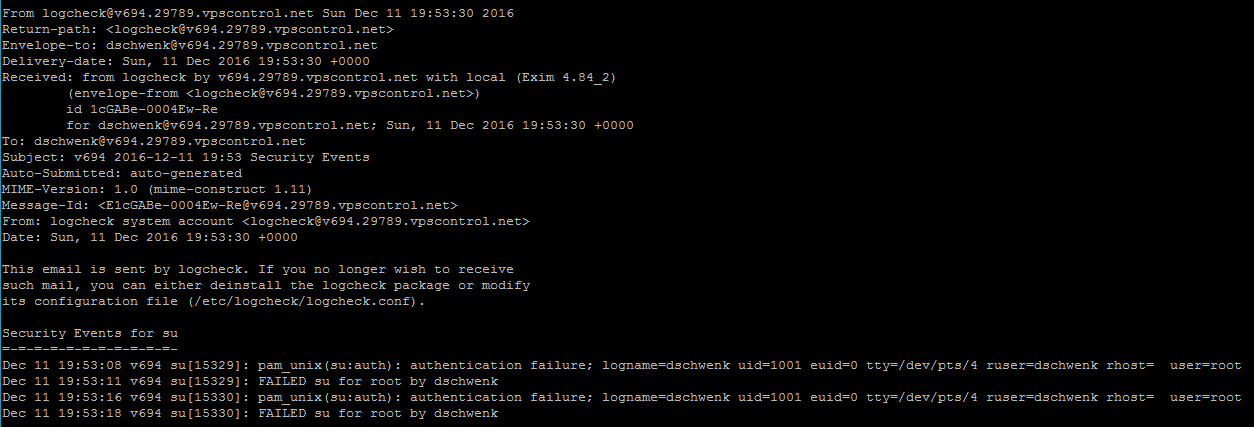
\includegraphics[width=1.0\textwidth]{img/logcheck_benachrichtigung.png}
	\caption{Beispielhafte \textit{logcheck}-Benachrichtigung einer fehlerhaften Authentifizierung}
	\label{fig:logcheck}
\end{figure}



\section{SSH-Honeypot}
\label{sec:SSH-Honeypot}

\subsection{Installation und Konfiguration Kippo}
\label{subsec:Installation und Konfiguration Kippo}

% vorgehenseise installation + konfiguration kippo\\
% http://www.blackhat.pm/ssh-honeypot-on-debian-with-kippo.html
% https://technik.blogbasis.net/kippo-ssh-honeypot-installieren-17-10-2014

% ausführliche Beschreibung Kippo + Dateien\\
% http://resources.infosecinstitute.com/tracking-attackers-honeypot-part-2-kippo/

Dieses Kapitel beschreibt die Vorgehensweise zur Installation und Konfiguration von einem SSH-Honeypot auf Basis von Kippo. Dieser SSH-Honeypot soll wie für SSH üblich auf Port 22 eingerichtet werden. Da aktuell der standard SSH-Dienst auf Port 22 läuft, muss dieser zuvor angepasst werden. Dazu wird der Port in der Konfigurationsdatei \textit{etc/ssh/sshd\_config} auf Port 10022 abgeändert und der Dienst anschließend neu gestartet.\\

Damit Kippo lauffähig ist, sind einige zusätzliche Pakete notwendig\footnote{ Kippo Abhängigkeiten: \url{https://github.com/desaster/kippo\#requirements}}. Diese werden, ebenso wie der git-Client für einen einfachen Download des Kippo-Projekts, über den Paketmanager installiert:

\begin{lstlisting}[style=customc]
apt-get install python-dev openssl python-openssl python-pyasn1 
  python-twisted git
\end{lstlisting}

Einer Ausführung von Befehlen oder Diensten mit root-Rechten sollte stets wohl bedacht sein und nach Möglichkeit vermieden werden. Die Ausführung des Honeypot-SSH-Dienstes mit root-Rechten oder auch unter einem unserer Benutzer wäre höchst sicherheitskritisch. Ein Angreifer könnte darüber volle Kontrolle über das Hostsystem erlangen. Um diese Gefahr möglichst gering zu halten wird ein separater Benutzer mit Homeverzeichnis, zugewiesener Shell und der sudo-Gruppenzugehörigkeit angelegt:

\begin{lstlisting}[style=customc]
useradd -d /home/kippo -s /bin/bash -g sudo
\end{lstlisting}

Um auf einem Linux-System einen Port kleiner 1024 ("`well known ports"') zu verwenden sind root-Rechte erforderlich. Genau dies soll für den SSH-Honeypot-Dienst wie oben beschrieben vermieden werden. Um auch einem normalen Benutzer die Verwendung eines Ports kleiner 1024 zu ermöglichen, wird auf das Programm \textit{AuthBind}\footnote{ \textit{AuthBind}: \url{http://man.cx/authbind(1)}} zurückgegriffen. Die Installation von Authbind erfolgt via:

\begin{lstlisting}[style=customc]
apt-get install authbind
\end{lstlisting}

Die Verwendung von Port 22 wird über die Erstellung einer Datei durch \textit{touch} unter \textit{/etc/authbind/byport/} sowie die Anpassung des Besitzes und der Berechtigungen für den Kippo-Benutzervia \textit{chown} und \textit{chmod} auf diese Datei ermöglicht:

\begin{lstlisting}[style=customc]
touch /etc/authbind/byport/22
chown kippo /etc/authbind/byport/22
chmod 777 /etc/authbind/byport/22
\end{lstlisting}

Der Download von Kippo erfolgt direkt von der Projektseite auf Github\footnote{ \textit{Kippo-Projekt auf Github}: \url{https://github.com/desaster/kippo}}:

\begin{lstlisting}[style=customc]
git clone https://github.com/desaster/kippo.git
\end{lstlisting}

Im Kippo-Verzeichnis befindet sich eine Datei, die eine Standardkonfiguration enthält. In dieser wird der  voreingestellte Port auf Port 22 abgeändert. Zudem muss die Konfigurationsdatei in \textit{kippo.cfg} umbenannt werden:

\begin{lstlisting}[style=customc]
mv kippo.cfg.dist kippo.cfg
\end{lstlisting}

Damit Kippo mit Hilfe von AuthBind ausgeführt wird, muss das "`Kippo-Start-Skript"' angepasst werden. Dazu wird der Befehl \textit{authbind} in das Skript aufgenommen:

\begin{lstlisting}[style=customc]
authbind --deep twistd -y kippo.tac -l log/kippo.log --pidfile kippo.pid
\end{lstlisting}

Der Parameter \textit{--deep} sorgt dafür, dass nicht nur das direkt folgende Programm, sondern auch alle Programme die folge dieses Aufrufs sind, unter \textit{authbind} ausgeführt werden. Kippo selbst basiert auf Twisted, einer "`Event-basierten Netzwerkengine"'\footnote{ \textit{Twisted - Building the engine of your internet}: \url{http://twistedmatrix.com/trac/}} für Python. twistd\footnote{ \textit{twistd}: \url{https://linux.die.net/man/1/twistd}} wird über den Parameter "`\textit{y}"' die Python-Applikation, zudem eine Logdatei sowie ein Pidfile übergeben. In diesem wird die Prozess-ID abgelegt.

Nach Ausführung des Kippo-Startskript \textit{start.sh} läuft der Prozess im Hintergrund. In Folge dessen wird auch das Kippo-Logfile angelegt, in dem Zugriffe auf den SSH-Honeypot-Dienst dokumentiert werden. Änderungen in diesem Logfile können über

\begin{lstlisting}[style=customc]
tail -f /home/kippo/kippo/log/
\end{lstlisting}

direkt verfolgt werden. \textit{tail} gibt über den Parameter automatisch neue Zeilen im Logfile auf der Kommandozeile aus. Von nun an kann auch eine Verbindung auf Port 22 aufgebaut werden. Nicht zu vergessen ist, dass der SSH-Dienst auf Port 10022, der die Verbindung der Projektmitarbeiter ermöglicht, durch einen Portscanner wie NMap aufgespürt werden kann.

\begin{figure}[ht]
	\centering
		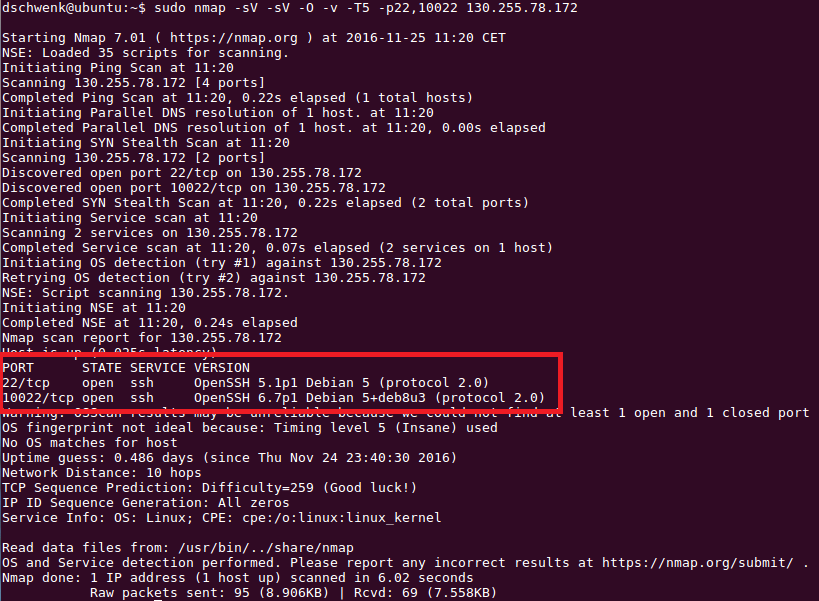
\includegraphics[width=1.0\textwidth]{img/nmap_ssh.png}
	\caption{Ausgabe Portscanner Nmap gegen das Honeypot-System}
	\label{fig:nmap_ssh}
\end{figure}

Das Kippo-SSH-Banner, welches in Abbildung \ref{fig:nmap_ssh} zu erkennen ist, kann über die Kippo-Konfigurationsdatei \textit{kippo.cfg} angepasst werden. In dieser Konfigurationsdatei können ebenfalls unter anderem folgende Einstellungen vorgenommen werden:

\begin{itemize}
\item Verzeichnis, in die Kippo eine Logdatei mit allen Aktivitäten schreibt. Alternativ kann eine Datenbank zur Protokollierung verwendet werden. Aus Zeit- und Performancegründen entscheidet sich das Projektteam für die Logdatei.
\item Angabe des Verzeichnisses, in dem die Datei \textit{fs.pickle} mit dem virtuellen Dateisystem liegt
\item Angabe einer Datei, die vordefinierten Antworten auf diverse Kommandos enthält. Die Ausgabe dieser Antworten erhält ein Angreifer nach einem erfolgreichen Login bei der Eingabe von Standardkommandos
\end{itemize}

Die Kombinationen an Benutzernamen und Passwörter, mit denen ein Login über den SSH-Honeypot möglich ist, kann in der Datei \textit{userdb.txt} spezifiziert werden. Standardmäßig ist hier der Benutzername \textit{root} mit dem Passwort \textit{123456} hinterlegt. Um einem Angreifer eine größere Angriffsfläche zu bieten, wird diese List um folgende Einträge ergänzt:

\begin{lstlisting}[style=customc]
root:123456
root:root
root:r00t
admin:123456
admin:admin
admin:password
\end{lstlisting}

Damit ist die Installation und grundlegende Konfiguration des SSH-Honeypots abgeschlossen.

\subsection{Kippo-Logfile auswerten}
\label{subsec:Kippo-Logfile auswerten}

% - extract uniq ips aus kippo logfile \\
% https://bruteforce.gr/extracting-unique-ips-from-logfile.html \\

Die IP-Adressen von Angreifern werden im Kippo.log-Logfile neben zahlreichen Informationen wie eingegeben Benutzernamen, Passwörter und Befehle gespeichert. Ein Auszug aus einem Kippo-Logfile ist im Anhang unter \textit{\nameref{app:Ausschnitt aus Kippo-Logdatei}} zu finden. Aus diesen Informationen sollen Statistiken zu Benutzernamen und Passwörter sowie automatisiert Firewallregeln erstellt werden, um Angriffe von diesen IPs zu verhindern.

Wie dem Kippo-Logfile unter \textit{\nameref{app:Ausschnitt aus Kippo-Logdatei}} zu entnehmen ist, werden Benutzernamen und Passwörter als Teile von Zeichenketten im Logfile abgelegt. Für eine Auswertung müssen diese aus dem Logfile extrahiert werden. Dies erfolgt mit Hilfe der Werkzeuge \textit{grep}, welches nach  einer gegebenen Zeichenkette, hier "`login attempt"', in einer Datei sucht. Die Zeilen, die dem Suchmuster entsprechen werden via Pipe an \textit{awk} übergeben. \textit{awk} arbeitet intern mit Variablen, die jeweils eine Zeichenkette einer Zeile, die voneinander durch Leerzeichen getrennt sind beinhalten. Die Variable sind dabei fortlaufend nummeriert. Variable \$0 enthält die ganze Zeile, Variable \$9 die neunte durch Leerzeichen getrennte Zeichenkette, die in diesem Fall den Loginnamen und das Passwort im Format "`[login/password]"' enthält. Duplikate werden durch \textit{sort} und \textit{uniq} entfernt. Über \textit{sed} und einen regulären Ausdruck werden die beiden eckigen Klammern entfernt:


% http://bob.k6rtm.net/kippowho.html

\begin{lstlisting}[style=customc]
grep ' login attempt ' kippo.log |
  awk '{print ($9)}' |
  sort |
  uniq |
  sed -r 's/]|\[//g' > user.txt

\end{lstlisting}

Hierdurch erhalten wir eine Liste von Kombinationen aus Benutzernamen und Passwörter in der Form \textit{username/passwort}. Passwörter werden zudem separat ohne Benutzernamen extrahiert. Dazu ist ein weiterer Aufruf von sed notwendig, der den Benutzernamen und das "`/"' entfernt. Passwortduplikate werden hierbei nicht entfernt, um daraus aussagekräftige Statistiken generieren zu können.

\begin{lstlisting}[style=customc]
grep ' login attempt ' kippo.log |
  awk '{print ($9)}' |
  sed "s|^.*/||g" |
  sed "s|]||g" > pw.txt
\end{lstlisting}

Die Ausführung dieser Befehle wird über ein Bash-Skript realisiert. Das vollständige Skript ist im Anhang unter \textit{\nameref{app:Benutzernamen und Passwörter extrahieren}} zu finden.
Die Auswertung der Passwörter erfolgt über \textit{Pipal Password Analyzer}\footnote{ \textit{Pipal Password Analyzer}: \url{https://github.com/digininja/pipal}}. Dieses open source Werkzeug erstellt Statistiken über die am häufigsten eingegeben Passwörter, über Zusammensetzung der Passwörter aus verschiedenen Zeichenklassen sowie Passwortlänge. Zudem erstellt es dazu "`Text-Grafiken"'. Der \textit{Pipal Password Analyzer} basiert auf \textit{ruby}, was durch \textit{apt-get install ruby} installiert wird. Der Download des Werkzeugs selbst erfolgt von der Projektseite auf Github:

\begin{lstlisting}[style=customc]
git clone https://github.com/digininja/pipal.git
\end{lstlisting}

Anschließend können Statistiken via

\begin{lstlisting}[style=customc]
pipal.rb /pfad/zur/passwortdatei Ausgabedatei
\end{lstlisting}

erzeugt werden. Eine dieser Statistiken ist im Anhang unter \textit{\nameref{app:Pipal Passwortstatistik}} zu finden.

%- Auswertung der Passwörter (diese müssen zuerst geparst werden)\\
% https://github.com/digininja/pipal
% https://digi.ninja/blog/pipal_kippo.php
% - alternativ Kippo Graph
% https://github.com/ikoniaris/kippo-graph

\subsection{Firewallregeln erstellen}
\label{subsec:Firewallregeln erstellen}

Ziel unseres System ist es, einen Angreifer zu beobachten und aus seinem Vorgehen zu lernen. Anschließend soll der Angreifer von der Infrastruktur fern gehalten werden, um die Sicherheit anderer Systeme zu wahren. Um einen Angreifer wirkungsvoll von einer Infrastruktur fernzuhalten, besteht die Möglichkeit den Datenverkehr des Angreifers mit einer Firewall, die dieser Infrastruktur vorgelagert ist, zu blockieren. Da in dem vorliegenden Versuchsaufbau keine weiterreichende Infrastruktur mit einer vorgelagerten Firewall vorhanden ist, wird hier exemplarisch auf dem Honeypotsystem selbst die Abwehr der Datenpakete des Angreifers mit Hilfe von \textit{iptables} vorgenommen. Die Wahl fällt auf \textit{iptables}, da hiermit Firwallregeln über sogenannte Ketten von Regeln erstellt werden können. Zudem ist \textit{iptables} standardmäßig unter Debian verfügbar und kann über ein Bash-Skript automatisiert werden. 

Um Firewallregeln generieren zu können, müssen die IP-Adressen der Angreifer aus dem Kippo-Logfile extrahiert werden. Dies geschieht wie bereits unter \ref{subsec:Kippo-Logfile auswerten} beschrieben mit Hilfe der Werkzeuge \textit{grep}, \textit{sort} und \textit{uniq}. Dazu wird an \textit{grep} ein regulären Ausdruck übergeben, der IP-Adressen filtert. Damit keine identischen Firewallregeln erzeugt werden, werden doppelte IP-Adressen über \textit{sort} und \textit{uniq} entfernt.

\begin{lstlisting}[style=customc]
cat logfile.log | 
  grep -o '[0-9]\{1,3\}\.[0-9]\{1,3\}\.[0-9]\{1,3\}\.[0-9]\{1,3\}' |
  sort |
  uniq > unique-ips.txt
\end{lstlisting}

Die Generierung der Firwallregeln geschieht über nachfolgendes Skript:

\begin{lstlisting}[language=bash,style=customccolor]
#!/bin/bash
#
# set variables
FW="/sbin/iptables"
IPFILE="/home/dschwenk/kippo-data/ips.txt"
BACKUPFILE="/home/dschwenk/firewall/iptables-backup.txt"

# backup current rules
iptables-save > $BACKUPFILE

# delete existing rules and chains
$FW -F
$FW -X

# set standard rules - accept all connections on all chains
$FW -P INPUT   ACCEPT
$FW -P FORWARD ACCEPT
$FW -P OUTPUT  ACCEPT

# read IP addresses from file
while read IP; do
  # drop connections from these IPs
  $FW -A INPUT -s $IP -j DROP 
done < $IPFILE


\end{lstlisting}

Das Skript fertig zuerst über \textit{iptabales-save} ein Backup der bestehenden Regeln an, welches wie unter \ref{sec:Archivierung und Automatisierung} beschrieben archiviert wird. Eine beispielhafte Ausgabe von \textit{iptables-save} ist im Anhang unter \textit{\nameref{app:Ausgabe iptables-save}} zu finden. Anschließend werden alle existierenden Regeln über die Parameter -F und -X gelöscht. Dies geschieht explizit, um keine doppelten Regelsätze zu erstellen. Dies würde die Performance von iptables unnötig mindern. Ebenfalls explizit werden über die Regeln standardmäßig alle Verbindungen für die INPUT-, FORWARD- und OUTPUT-Chain akzeptiert. Damit lassen sich aus den Verbindungs-Logfiles beispielsweise Portscans nachweisen. Die Regeln selbst werden über eine Schleife erstellt, die Zeilenweise die IP-Adressen aus der oben generierten Datei ausließt und alle Verbindungen dieser IP auf der INPUT-Chain verwirft. Dieses Skript wird über einen cronjob einmal täglich ausgeführt.



\subsection{IP-Adressen auswerten}
\label{subsec:IP-Adressen auswerten}

Unter \ref{sec:Kann-Kriterien} wurde eine Anforderungen für einen reverse-DNS-Lookup von Angreifer IP-Adressen aufgeführt. Die Angreifer-IP-Adressen wurde bereits durch das Skript unter \ref{subsec:Firewallregeln erstellen} extrahiert. Mit \textit{getent}\footnote{ \textit{getent}: \url{http://man7.org/linux/man-pages/man1/getent.1.html}} kann von diesen nun ein reverse-lookup erfolgen. Um dies nicht von Hand machen zu müssen, wird ein Skript erstellt:

\lstinputlisting
    [caption={Skript zur Extraktion von Benutzernamen und Passwörter aus Kippo-Logfile}
       \label{lst:reverse_dns},
       captionpos=b,language=bash,style=customccolor]
 {listings/do_reverse_dns_lookup.sh}

Eine beispielhafte reverse-DNS-Auswertung ist im Anhang unter \textit{\nameref{app:Auswertung reverse-DNS-Lookup}} zu finden.
Um nicht nur eine Zuordnung von IP-Adressen zu DNS-Namen zu haben, sondern um auch ein Gefühl für die Herkunft der Angriffe zu bekommen, entschied sich das Projektteam zusätzlich zu einer geographischen Darstellung. Die Website batchgeo.com\footnote{ batchgeo.com: \url{http://de.batchgeo.com/}} bietet einen Dienst, der anhand von gegeben Daten eine Karte erstellt. Diese gegeben Daten können beispielsweise Adressen, Koordinaten oder eben auch IP-Adressen sein. Mit Hilfe einer "`Geo-IP-Adressen-Funktion"' erstellt dieser Dienst eine Karte, auf der die IP-Adressen eingezeichnet sind. Abbildung \ref{fig:geo_ip_world} zeigt eine dieser erzeugten Karten, die die gesamte Welt abbildet.

\begin{figure}[ht]
	\centering
		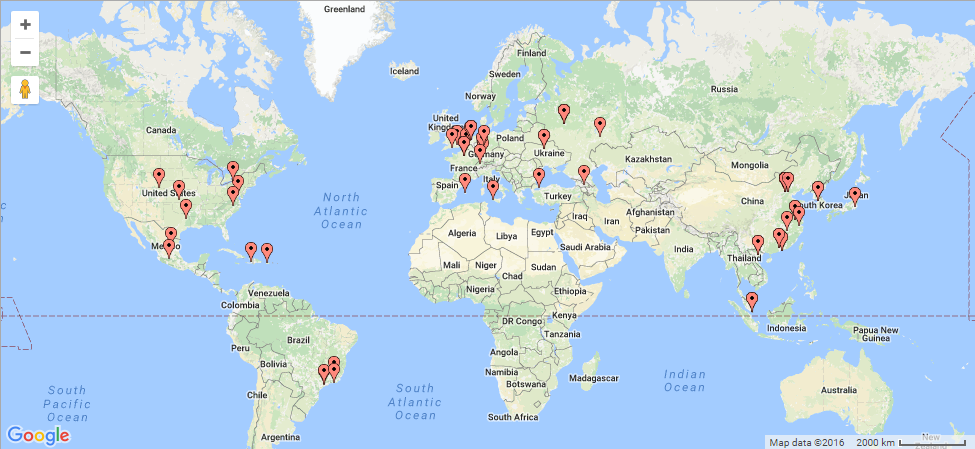
\includegraphics[width=0.94\textwidth]{img/geo_ip_world.png}
	\caption{Karte mit Geo-Location von Angreifer-IP-Adressen}
	\label{fig:geo_ip_world}
\end{figure}

Diese Karte zeigt deutliche, dass ein Großteil der Angriffe aus China, Europa und Nordamerika stammen. Abbildung \ref{fig:geo_ip_eu} zeigt speziell einen Ausschnitt von Europa:

\begin{figure}[ht]
	\centering
		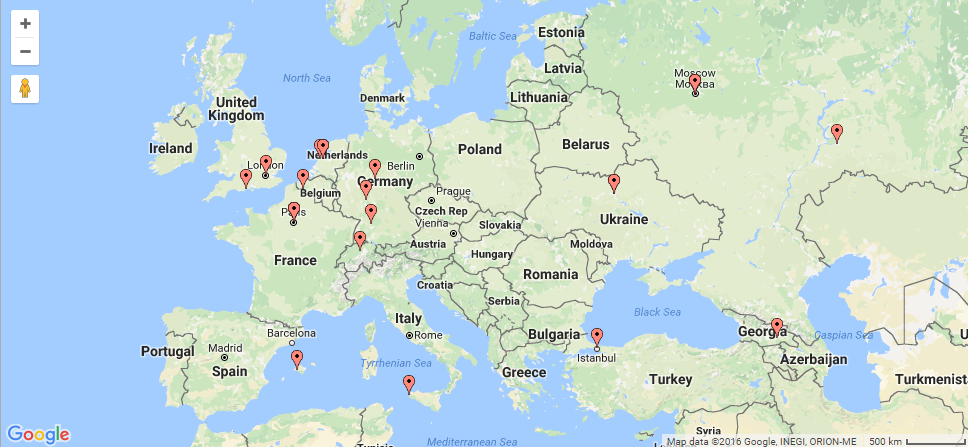
\includegraphics[width=0.94\textwidth]{img/geo_ip_eu.png}
	\caption{Karte mit Geo-Location von Angreifer-IP-Adressen}
	\label{fig:geo_ip_eu}
\end{figure}

Die Verteilung der IP-Adressen in Europa erstreckt sich hauptsächlich über Mitteleuropa. Allgemein muss diese Auswertung jedoch mit Vorsicht betrachtet werden, da die Zuordnung einer IP-Adresse zu einer Örtlichkeit einer gewissen Fehlerrate unterliegt. batchgeo.com ordnet die IP-Adresse mit Hilfe von Daten von MaxMind zu. MaxMind gibt für die Zuordnung von IP-Adressen zu Städten in Ländern wie den USA, China, Russland oder Deutschland eine Zuverlässigkeit von über 75\% an. Für andere Länder ist teilweise eine niedrigere Zuverlässigkeit gegeben, die in einigen Fällen unter 50\% liegt. Eine Auflistung je Land kann auf der Website von MaxMind\footnote{ MaxMind GeoIP2 City Accuracy: \url{https://www.maxmind.com/en/geoip2-city-database-accuracy}} eingesehen werden.



\subsection{Benachrichtigung bei Zugriff auf SSH-Honeypot}
\label{subsec:Benachrichtigung bei Zugriff auf SSH-Honeypot}

Unter \ref{sec:Kann-Kriterien} wurde eine Anforderung zur automatischen Benachrichtigung bei einem Angriff dokumentiert. Das Projektteam hat sich dazu entschieden, diese Benachrichtigung in Form einer Email-Benachrichtigung umzusetzen. Angedacht ist, eine Email dann zu versenden, wenn sich die Kippo-Logdatei ändert. Um nicht bei jeder Änderung benachrichtigt zu werden, soll in einem festen Zeitintervall auf Änderungen geprüft werden. Veränderungen an Dateien oder Verzeichnissen können unter Linux unter anderem mit \textit{inotifywait}\footnote{ \textit{inotifywait}: \url{https://linux.die.net/man/1/inotifywait}} überwacht werden. \textit{inotifywait} ist in dem Paket \textit{inotify-tools} enthalten, welches über

\begin{lstlisting}[language=bash,style=customccolor]
apt-get install inotify-tools 
\end{lstlisting}

installiert wird. Als Zeitintervall, in der auf Änderungen überprüft werden soll, wurde eine Stunde festgelegt. Dazu wird ein cronjob eingerichtet, der stündlich \textit{inotifywait} ausführt.

\begin{lstlisting}[language=bash,style=customccolor]
@hourly inotifywait -t 3599 -e modify /home/kippo/kippo/log/kippo.log && /home/dschwenk/email-alert/alert.sh
\end{lstlisting}

Als Parameter werden \textit{inotifywait} eine Zeit von 3599 Sekunden übergeben, damit sich dieser Prozess nach Ablauf dieser Zeit automatisch beendet. Würde keine Zeit angegeben werden, würde dieser Prozess bis zu einer Änderung, die in einer beliebigen Zeit in der Zukunft liegen kann, im Hintergrund weiter laufen. Stündlich würde jedoch zusätzlich ein neuer Prozess gestartet werden. Die Zeitangabe verhindert somit die Mehrfachausführung. Zusätlich wird die zu überwachende Logdatei angegeben, so wie eine Aktion, die bei einer Änderung ausgeführt werden soll. In diesem Fall soll das Skript \textit{alert.sh} ausgeführt werden, welches nachfolged aufgelistet ist:

\begin{lstlisting}[language=bash,style=customccolor]
#!/bin/bash

echo "Someone accessed our SSH honeypot running on port 22" | mailx -v \
-r "honeypot-notification@danielschwenk.de" \
-s "SSH Honeypot Notification" \
-S smtp="send.one.com" \
-S smtp-use-starttls \
-S smtp-auth=login \
-S smtp-auth-user="honeypot-notification@danielschwenk.de" \
-S smtp-auth-password="password" \
-S ssl-verify=ignore \
michael.stroh@hs-weingarten.de,daniel.schwenk@hs-weingarten.de
\end{lstlisting}

Dieses Skript sendet eine Email mit vorgegebenem Betreff und Inhalt an die beiden Projektmitglieder. Der Versand selber wird über \textit{mailx}\footnote{ \textit{mailx}: \url{https://linux.die.net/man/1/mailx}} realisiert, welches über

\begin{lstlisting}[language=bash,style=customccolor]
sudo apt-get install heirloom-mailx
\end{lstlisting}

installiert wurde. Dem \textit{mailx}-Kommando werden dazu die SMTP- und Benutzerdaten übergeben. Der Versand erfolgt mit Hilfe eines Emailaccounts, welcher beim Provider one.com\footnote{ one.com \url{https://www.one.com/de/}} angelegt wurde. Die Wahl fiel auf diesen Provider, da dieser bereits in anderen Projekten in Verwendung der Teammitglieder ist. Das in diesem Listing dargestellte Passwort wurde aus Sicherheitsgründen durch einen Platzhalter ersetzt.


\section{Web-Honeypot}
\label{sec:Web-Honeypot}

\subsection{Installation und Konfiguration SNARE}
\label{subsec:Installation und Konfiguration SNARE}

In diesem Abschnitt wird die Installation und Konfiguration eines Web-Honeypots auf Basis von SNARE beschrieben. Die Einrichtung erfolgt für Port 80 HTTP. 

\begin{lstlisting}[style=customc]
sudo apt-get install python3 python3-pip
\end{lstlisting}

Unter anderem wird Python3 für eine erfolgreiche Inbetriebnahme vorausgesetzt. Da zusätzlich noch mehrere Python-Module geladen werden müssen, bedarf es darüber hinaus des zugehörigen  Paketverwaltungsprogramms pip\footnote{ \textit{pip}: \url{https://pip.pypa.io/en/stable/}}, auch in der entsprechenden Version 3.

\begin{lstlisting}[style=customc]
pip3 install aiohttp beautifulsoup4 cssutils gitpython
\end{lstlisting}

Über das Paketverwaltungsprogramm werden daraufhin die Python-Module  installiert.

\begin{lstlisting}[style=customc]
apt-get install git
\end{lstlisting}

Falls nicht bereits systembedingt bereitgestellt, ist es an dieser Stelle zwingend erforderlich die Versionsverwaltungssoftware git\footnote{ \textit{git}: \url{https://git-scm.com/}} zu installieren.

\begin{lstlisting}[style=customc]
cd /home/mstroh/
git clone https://github.com/mushorg/snare.git
\end{lstlisting}

Über Github kann SNARE\footnote{ \textit{SNARE-Projekt auf Github}: \url{https://github.com/mushorg/snare}} bezogen werden.

\begin{lstlisting}[style=customc]
cd /home/mstroh/snare
sudo python3 clone.py --target http://example.com
\end{lstlisting}

SNARE stellt dabei selbst ein Skript bereit um bestehende Webpräsenzen zu klonen. Diese Klone werden unter
\begin{lstlisting}[style=customc]
/opt/snare/pages
\end{lstlisting}
abgelegt. Wahlweise kann natürlich auch eine eigene Webseite erzeugt und über SNARE gestartet werden.

\begin{lstlisting}[style=customc]
sudo python3 snare.py --interface eth0 --port 80 --page-dir example.com >> snare.log &
\end{lstlisting}
Die sudo-Rechte benötigt SNARE um den Python-HTTPRequestHandler an Port 80 zu binden. Direkt nachdem das geschehen ist, werden diese Privilegien wieder abgegeben und der Web-Honeypot selbst läuft unter einem eigens hierfür angelegten nicht privilegierten Nutzer. In der Standardkonfiguration heißt dieser Nutzer nobody. Über die Parameter \grqq{}--interface\grqq{} und \grqq{}--port\grqq{} werden Interface und Port für den Web-Honeypot festgelegt. \grqq{}--page-dir\grqq{} lädt die entsprechend zuvor geklonte oder selbst erzeugte Webseite und simuliert daraufhin einen Webserver. 

Sämtliche Zugriffe, auch solche, die aufgrund einer nicht vorhandenen Ressource scheitern, Nutzer-Eingaben und Zugriffsversuche werden von SNARE über die Python-Anweisung print ausgegeben. Über \grqq{}>> snare.log\grqq{} werden diese Ausgaben an das Logfile \grqq{}snare.log\grqq{} angehängt.  Ohne weiteres Zutun würden diese Ausgaben zum jeweiligen Ereigniszeitpunkt im Zwischenspeicher der Datei \grqq{}snare.log\grqq{} verbleiben und erst bei einer größer anfallenden Menge an Log-Einträgen tatsächlich in das Log-File geschrieben werden. Um der Anforderung einer automatischen Benachrichtigung bei einem stattfindenden Angriff gerecht werden zu können, hat sich das Projektteam dazu entschlossen, die Ausgaben des Skriptes zu erweitern und den bereitgestellten Zwischenspeicher zu umgehen, um Ereignisse unmittelbar im Log-File festzuhalten und entsprechend zeitnah auf etwaige Aktivitäten reagieren zu können. 

\begin{lstlisting}[style=customc]
print(.., flush=True)
\end{lstlisting}

Das Skript wurde an entsprechenden Stellen um diesen Parameter erweitert.

\begin{figure}[ht]
	\centering
		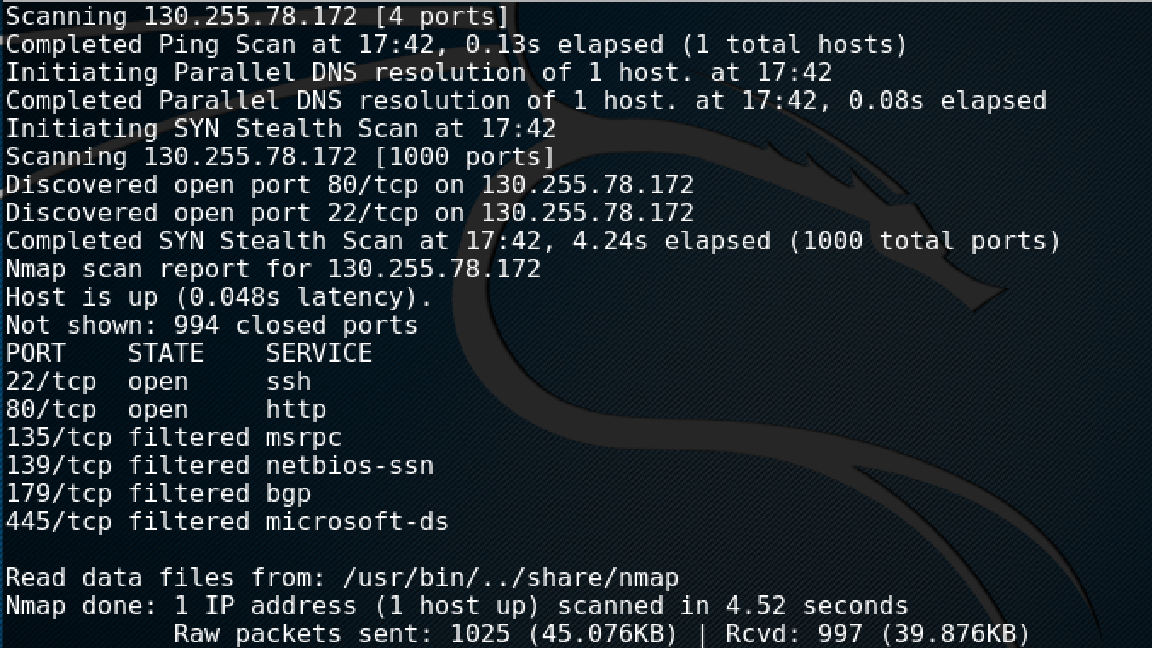
\includegraphics[width=1.0\textwidth]{img/nmap_web.png}
	\caption{Ergebnis eines Port-Scans mit Nmap nach zusätzlicher Inbetriebnahme des Web-Honeypots SNARE}
	\label{fig:nmap_web}
\end{figure}

Nach erfolgreichem Start von SNARE ist der Web-Honeypot über das zuvor angegebene Interface und den entsprechenden Port, hier 80, erreichbar.

\subsection{Verwendung eines Login-Formulars}
\label{subsec:Installation und Konfiguration SNARE}

Um einem Angreifer zusätzliche Angriffsfläche zu bieten, hat sich das Projektteam nach einwöchigem Betrieb einer Kopie von example.com\footnote{ example.com \url{http://www.example.com}} dazu entschlossen, eine Weboberfläche in Form eines Login-Formulars zu einzusetzen.

\begin{figure}[ht]
	\centering
		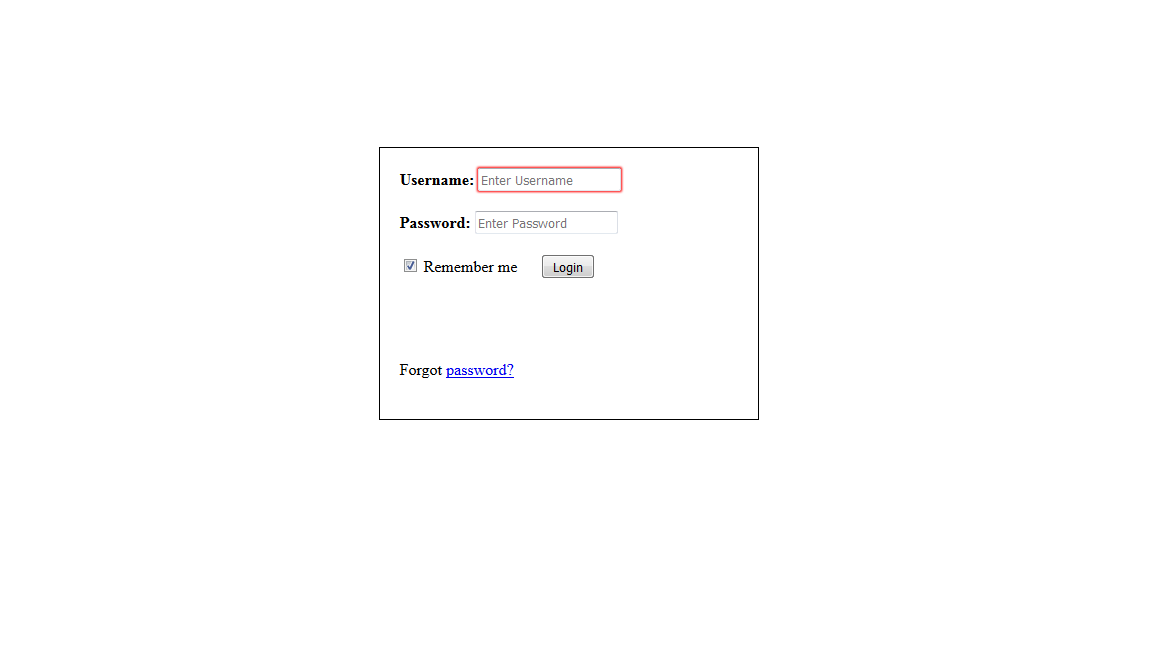
\includegraphics[width=1.0\textwidth]{img/snare_login.png}
	\caption{Weboberfläche des Web-Honeypots SNARE}
	\label{fig:snare_login}
\end{figure}

Dieses Login-Formular, wie Abbildung \ref{fig:snare_login} ersichtlich, besteht aus lediglich zwei Eingabefeldern für jeweils Benutzername und Passwort.

\subsection{SNARE-Logfile auswerten}
\label{subsec:Installation und Konfiguration SNARE}

SNARE loggt sämtliche HTTP-Anfragen in Form des angeforderten Pfades und zusätzlich eingehende HTTP-POST-Anfragen.

\begin{figure}[ht]
	\centering
		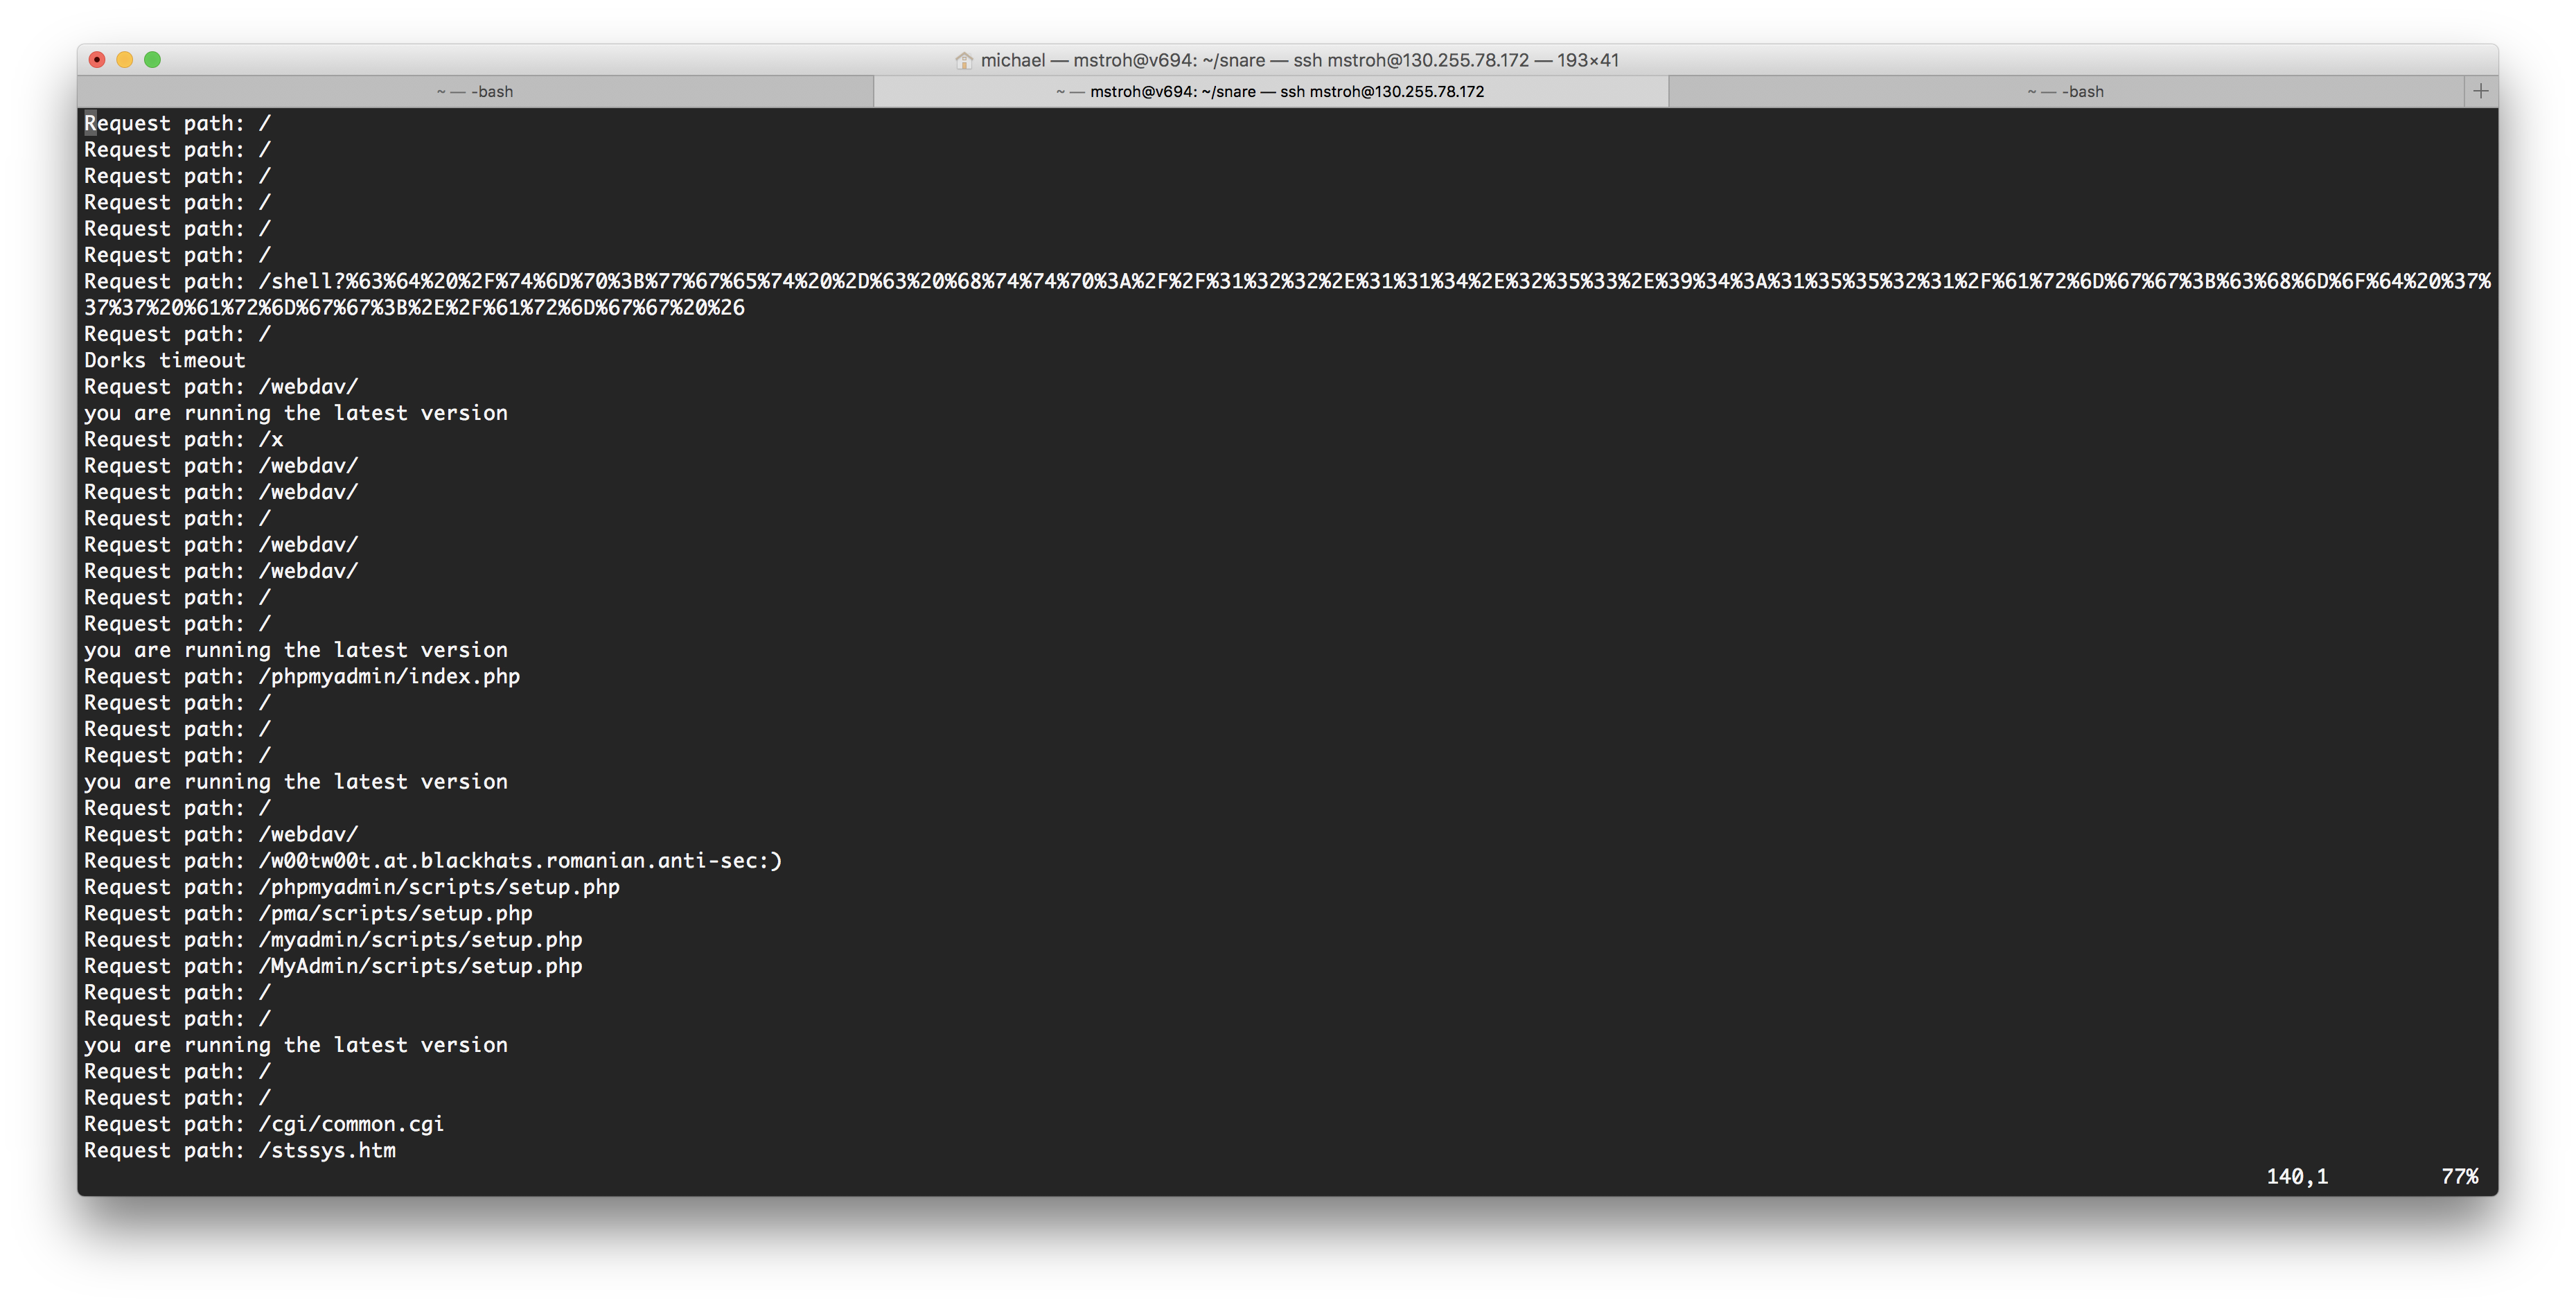
\includegraphics[width=1.0\textwidth]{img/snare_logfile.png}
	\caption{Auszug aus dem Log-File des Webhoneypots SNARE nach einwöchigem Betrieb}
	\label{fig:snare_logfile}
\end{figure}

Wie in Abbildung \ref{fig:snare_logfile} ersichtlich, werden angeforderte Pfade mit dem Präfix \grqq{}Request path:\grqq{} und POST-Anfragen mit \grqq{}POST data:\grqq{} versehen. Da zusätzliche, ebenfalls in diesem Log-File gesicherte Programm-Ausgaben, wie etwa die zum Systemstart verwendeten Parameter, für das Projektteam irrelevant sind, werden für eine weitere Unterteilung lediglich die zwei zuvor genannten Kategorien verwendet.


\begin{lstlisting}[style=customc]
grep 'POST data:' snare.log |
tr -s '\n' |
sort |
uniq -ic |
sort -gr > snare-post-requests.txt
\end{lstlisting}

Unter Verwendung von grep werden alle Einträge, die durch einen HTTP-POST entstanden sind, welche durch die vorangestellte Ausgabe 'POST data:' identifiziert werden, herausgefiltert. 'tr -s' entfernt daraufhin mehrere aufeinanderfolgende Zeilenumbrüche. Mittels 'sort' wird das Ergebnis entsprechend der Zeichenfolge des jeweiligen Eintrags sortiert und durch 'uniq -ic' werden mehrere gleiche Einträge zu einem einzigen Eintrag zusammengefasst, die Groß- und Kleinschreibung wird dabei ignoriert und die Anzahl der Vorkommnisse eines Eintrages durch den Parameter 'c' gezählt und jeweils als Ganzzahl vorangestellt. Dieses Ergebnis wird daraufhin noch einmal entsprechend der Häufigkeit('sort -g') und in absteigender Reihenfolge('sort -r') sortiert.

\begin{lstlisting}[style=customc]
grep 'Request path:' snare.log |
tr -s '\n' |
sort |
uniq -ic |
sort -gr > snare-path-requests.txt
\end{lstlisting}

Durch die gleiche Vorgehensweise werden auch alle angeforderten Pfade extrahiert. Um eine statistische Auswertung durchführen zu können.

Diese Befehle werden mit Hilfe eines hierfür geschriebenen Bash-Skripts ausgeführt, welches im Anhang unter \textit{\nameref{app:POST- und Path-Requests extrahieren}} eingesehen werden kann.


\subsection{Benachrichtigung bei Zugriff auf Web-Honeypot}
\label{subsec:Installation und Konfiguration SNARE}

Aufgrund von Erfahrungen bei der Verwendung einer automatischen Benachrichtigung bei dem SSH-Honeypot Kippo, hat sich das Projektteam dazu entschlossen, beim Web-Honeypot drei Mal täglich auf Veränderungen des Log-Files zu prüfen und die Projektmitglieder über neue Einträge in Kenntniss zu setzen.


\section{Archivierung und Automatisierung}
\label{sec:Archivierung und Automatisierung}


\subsection{Archivierung von Daten auf Cloud-Speicher}
\label{subsec:Archivierung von Daten auf Cloud-Speicher}

Um der Soll-Anforderung nach der Archivierung von Logdaten sowie Analyseergebnisse zu entsprechen, werden diese Daten automatisiert auf einem Cloud-Speicher abgelegt. Dieses Archivierung stellt sicher, dass auf diese Daten selbst dann zurückgegriffen werden kann, wenn das System kompromittiert wurde oder nicht weiter zur Verfügung steht. Eine Marktanalyse ergibt eine Vielzahl an verfügbaren Cloud-Speichern. Das Projektteam entscheidet sich auf Grund der Verfügbarkeit eines Linux-Clients, der einfachen Installation und Konfiguration dieses Clients sowie dessen Möglichkeit zur automatischen Ausführung via Kommandozeile für Google Drive\footnote{ Google Drive: \url{https://www.google.com/intl/de_de/drive/}}. Anzumerken ist, dass dieser Client nicht von Google selbst, sondern von Petter Rasmussen in einem open source Projekt entwickelt wird\footnote{ Peter Rasmussen gDrive command line tool: \url{https://github.com/prasmussen/gdrive}}. Der Download der aktuellen Version 2.1 des 64-Bit-Clients für Linux erfolgt durch:

\begin{lstlisting}[style=customc]
wget https://docs.google.com/uc?id=0B3X9GlR6EmbnQ0FtZmJJUXEyRTA&export=download
\end{lstlisting}

Durch eine Umbennung wird der kryptische Dateiname lesbar gemacht. Zudem wird die Datei als ausführbar markiert:

\begin{lstlisting}[style=customc]
mv 0B3X9GlR6EmbnQ0FtZmJJUXEyRTA&export gdrive
chmod +x gdrive
\end{lstlisting}

Die Installation erfolgt via:

\begin{lstlisting}[style=customc]
sudo install gdrive /usr/local/bin/gdrive
\end{lstlisting}

Nach der erfolgreichen Installation des Clients müssen diesem Berechtigungen zum Zugriff auf einen Google Drive Account eingerichtet werden. Dazu wird der Client mit einem beliebigen Parameter, hier \textit{list} zum Auflisten der gdrive-Inhalte, aufgerufen:

\begin{lstlisting}[style=customc]
gdrive list
\end{lstlisting}

Infolge dessen wird eine Aufforderung zum Besuch der Google-Drive-Website zur Authentifizierung ausgegeben. Somit ist eine Verbindung zwischen dem Client und dem Google Drive-Dienst hergestellt. Das Backup selbst wird über das Skript unter \ref{subsec:Automatisierung} erstellt und hochgeladen.


\subsection{Automatisierung}
\label{subsec:Automatisierung}

In den vorherigen Kapitel wurde die Vorgehensweise zur Extraktion, Auswertung und Weiterverarbeitung von Daten erläutert. Für einzelne Aufgaben wurden dazu Skripte erstellt. Um diese Skripte nun nicht regelmäßig von Hand ausführen zu müssen, werden diese einzelne Skripte über ein zentrales Skript gesteuert und täglich ausgeführt. Dieses Skript führt folgende Aufgaben aus:

\begin{itemize}
\item Daten aus Kippo-Logdatei extrahieren
\item Daten aus SNARE-Logdatei extrahieren
\item extrahierte Daten auswerten
\item bestehende Firewallregeln sichern sowie neue Regeln erstellen
\item Archivierung von Logdaten sowie Analyseergebnissen
\end{itemize}

In die Archivierung fließen sämtliche Log- und Analysedaten sowie Konfigurationsdateien ein. Dazu gehören:

\begin{itemize}
\item Kippo-Konfiguration und Logdatei
\item SNARE-Konfiguration und Logdatei
\item Auswertung der Benutzer- und Passwortdaten
\item Auswertung der IP-Adressen
\item Konfigurationsdateien von iptables
\item Auswertung der SNARE-Logdatei
\end{itemize}

Für einen effizienten Upload werden die oben genannten Dateien alle 24 Stunden zu einem komprimierten zip-Archiv zusammengefasst und auf den Cloud-Speicher hochgeladen. Um diesen Vorgang zu automatisieren wird folgendes Bash-Skript angelegt:

\lstinputlisting
    [caption={Skript zur Extraktion von Benutzernamen und Passwörter aus Kippo-Logfile}
       \label{lst:mitm_onmsg},
       captionpos=b,language=bash,style=customccolor]
 {listings/do_all.sh}
 
Dieses Skript soll täglich ausgeführt werden. Dies kann über einen \textit{cronjob} erreicht werden. Da für die Konfiguration von Firewallregeln via \textit{iptbles} root-Berechtigungen notwendig sind, muss dieses Skript mit privilegierten Berechtigungen ausgeführt werden. Über \textit{sudo crontab -e} wird ein \textit{cronjob} für den root-Benutzer eingerichtet:

\begin{lstlisting}[style=customc]
@daily /home/dschwenk/do_all_stuff.sh
\end{lstlisting}

Damit wird das Skript einmal täglich ausgeführt.

\chapter{Evaluation}
\label{ch:Evaluation}

\section{Umsetzung der Anforderungen}
\label{sec:Umsetzung der Anforderungen}

Die unter \ref{sec:Muss-Kriterien} aufgeführten Muss-Kriterien wurden vollständig erfüllt. In diesem Projekt wurde ein Honeypotsystem auf einem von providerdienste.de bereitgestellten vServer umgesetzt. Dieser vServer ist über eine öffentliche IPv4-Adresse im Internet erreichbar und implementiert einen SSH- und Webhoneypot. Durch die von providerdienste.de bereitgestellte Konsole ist es möglich, das System selbst dann, wenn keine Verbindung via SSH möglich ist oder der Server kompromittiert oder gar übernommen wurde, zu konfigurieren und darauf zuzugreifen. Es ist dem Projektteam somit jederzeit möglich, das Honeypotsystem abzuschalten, sofern die Situation es erfordern sollte. Durch die Aktualisierung aller Pakete und der Limitierung der SSH-Authentifzierung auf ein Public-Key-Verfahren wurde das Honeypotsystem bestmöglich abgesichert. Jeglicher Datenverkehr wird geloggt. Einem Angreifer ist es somit ohne den Besitz eines der Private-Keys der Projektmitglieder, Kenntnisse über aktuelle Schwachstellen bei den eingesetzten Systemen oder Infiltration des Rechenzentrums von providerdienste.de, nicht ohne Weiteres möglich sich Zugriff zu dem eingesetzten vServer zu verschaffen. Die Möglichkeit zur Manipulation von protokollierten Daten ist somit, gemessen an den zeitlichen Ressourcen des Projektteams, kleinstmöglich gehalten.\\

Das Soll-Kriterium der automatischen Benachrichtigung bei einem Angriff auf das Honeypotsystem stellte sich im Nachhinein als nicht sonderlich hilfreich dar. Speziell auf Port 22 und somit auf den SSH-Honeypot wurden täglich viele Verbindungen aufgebaut. Die Benachrichtigung darüber war für die Projektmitglieder aber wenig hilfreich, da jegliche Kommunikation und Angriffsversuche geloggt und automatisiert ausgewertet wurden. Zudem werden die auswerteten Daten und Konfigurationen automatisch über eine verschlüsselte Verbindung auf dem Cloud-Speicher Google Drive abgelegt. Die Benachrichtigung bietet so nur einen geringen Mehrwert. Bei der Archivierung der auswerteten Daten sowie dem Backup von Konfigurationsdateien ist anzumerken, dass hier ein separater Server oder ein anderes Backupmedium möglicherweise besser geeignet wäre, da es mit den Richtlinien von Google zu einem Datenschutzkonflikt kommen kann.\\

Der Soll-Anforderung einer automatisierten Auswertung von Logdaten wurde durch den Einsatz selbstgeschriebener Bash-Skripte, sowie der fertigen Lösung Pipal zur statistischen Analyse von Passwörtern entsprochen. Ebenso der automatisiert stattfindenden externen Sicherung sowohl von Log-Files selbst als auch den Log-Files zugehörige, bereits ausgewertete Daten wurde entsprochen, indem diese unter Verwendung eines Bash-Skripts auf Google-Drive hochgeladen. 

Die Kann-Kriterien unter \ref{sec:Kann-Kriterien} wurden nur teilweise erfolgreich umgesetzt. So war es dem Projektteam aus technischen Gründen nicht möglich, neben dem Honeypotsystem weitere Systeme wie einen Router, eine Firewall oder PCs in die Infrastruktur zu integrieren. Auch die Umsetzung eines Honeypots, der ein offenes WLAN oder einen Fake-Acces-Point bietet konnte nicht umgesetzt werden. Hier bietet sich Verbesserungspotential, da die durch ein Honeypot gewonnen Informationen speziell in einer größeren Umgebung wertvoll sind. So ist denkbar, aus den gesammelten IP-Adressen Firwallregeln zu erstellen, die auf einer der Infrastruktur vorgelagerten Firewall zur Wirkung kommen.
Die komplette Umsetzung des Projekts fand auf einem gemieteten vServer statt. Die Kosten liegen hier mit 9,00 Euro je Monat in einem überschaubaren Rahmen. Die Anforderung nach einem geringen Stromverbrauch kann nicht exakt beurteilt werden, da über den Stromverbrauch keine Informationen vorliegen. Auf Grund dessen, dass es sich bei unserem System um ein virtuelles System handelt, welches sich ein physikalisches System mit anderen virtuellen Systemen teilt, kann jedoch von einer gewissen Energieeffizienz ausgegangen werden. Die Anforderung an einen reverse DNS-Lookup wurde wie unter x.y beschrieben umgesetzt und zusätzlich durch eine Darstellung einer Geo-IP-Karte (siehe Anhang x.y) ergänzt

\section{Schlussfolgerungen SSH-Honeypot}
\label{sec:Schlussfolgerungen SSH-Honeypot}

Wie der Statistik im Anhang unter \nameref{app:Pipal Passwortstatistik} entnommen werden kann, wurden am SSH-Honeypot-Port ingesamt 420 Passwörter eingegeben, 130 davon sind einzigartig. Die 10 meistgenutzten Passwörter machen 35,46\% aller Passworteingaben aus. Betrachtet man die 10 meistgenutzten Passwörter genauer, fällt auf, das hier vorrangig die Zeichenketten \textit{admin} und \textit{password} sowie Zahlenfolgen wie \textit{123456} vertreten sind. Die Länge der eingegeben Passwörter betrug in über 25\% der Fälle sechs Zeichen, in 15,71\% acht Zeichen und in 14,29\% vier Zeichen. Über 80\% der eingegeben Passwörter bestanden aus acht oder weniger Zeichen. Ähnlich klare Verteilungen sind bei der Zusammensetzung von Passwörter aus Zeichenklassen zu erkennen. So bestehen über 38\% der Passwörter rein aus Buchstaben, weitere 30,48\% rein aus Zahlen.\\

Eine ähnliche einseitige Verteilung lässt sich bei den verwendeten Benutzernamen erkennen. In über 50\% der Fälle wurde der Benutzername \textit{root} verwendet. Werden die Benutzernamen \textit{admin}, \textit{user} und \textit{test} hinzugezählt, decken diese Benutzernamen über 75\% ab.\\

Aus diesen Zahlen wird vor allem eines deutlich. Die Verwendung eines der oben genannten Passwörter in Verbindung mit einem der genannten Benutzernamen birgt ein erhebliches Sicherheitsrisiko. Werden die Zugriffszeiten der Angreifer auf den SSH-Honeypot berücksichtigt, kann bei der Verwendung dieser Benutzer-Passwort-Kombinationen von einer Kompromittierung innerhalb weniger Stunden oder gar Minuten ausgegangen werden. Es sollte so zwingend sichergestellt werden, dass ein sicheres Passwort verwendet wird. Besser ist die Authentifizierung rein auf das Public-Key-Verfahren zu beschränken.\\

Es muss angenommen werden, dass Angreifer nicht nur bei SSH-Zugriffen auf einfache Kombination aus Benutzernamen und Passwörter setzen. Jedoch ist bei anderen Diensten zur Passwortauthentifizierung oftmals keine Alternative vorgesehen. In diesem Fall sollte zwingend ein sicheres Passwort gewählt werden. Um die Definition eines sicheren Passworts zu veranschaulichen, leitet das Projektteam aus der Passwortstatistik eine Passwortrichtlinie ab. Diese sieht vor, dass ein sicheres Passwort folgende Eigenschaften besitzt:

\begin{itemize}
\item Passwortlänge von mindestens 10 oder mehr Zeichen
\item Kombination aus den Zeichenklassen Klein- und Großbuchstaben, Zahlen und Sonderzeichen
\item Benutzung von Wörtern und persönlichen Daten wie Namen und Geburtsdatum vermeiden
\end{itemize}

Da selbst im Bewusstsein dieser Richtlinien dazu tendiert wird, nicht sichere Passwörter zu genieren, empfiehlt das Projektteam die Verwendung eines Passwortmanagers wie KeePass\footnote{ \textit{KeePass}: \url{http://keepass.info/}}. KeePass ist für alle gängigen Betriebssysteme verfügbar und ermöglicht es rein zufällige Passwörter zu generieren, zu verwalten und sicher zu speichern. Somit kann auch der Empfehlung für jeden Dienst ein separates Passwort zu verwenden einfach nachgekommen werden.

\section{Schlussfolgerungen Web-Honeypot}
\label{sec:Schlussfolgerungen Web-Honeypot}

Innerhalb eines Zeitraumes von einer Woche erfolgten auf dem Web-Honeypot 149 Zugriffe über HTTP und 5 POST-Requests. Angeforderte Pfade und POST-Requests können im Anhang unter \nameref{app:Auswertung snare-path-requests} und \nameref{app:Auswertung snare-post-requests} eingesehen werden. Während dieses Zeitraums bestand der Webauftritt des Web-Honeypots aus einer Kopie der Seite example.com\footnote{ \textit{example.com}: \url{http://example.com/}}. Ungeachtet der Tatsache, dass damit einem Angreifer lediglich die Möglichkeit gegeben war über verschiedene Pfade einen Zugriff zu potentiell über die Startseite nicht erreichbaren Login Seiten zu erhalten oder über Anwendung von HTTP-Methoden wie POST Schadcode einschleusen zu können und somit die angebotene Angriffsfläche sehr gering ausfiel, konnte das Projektteam mehrere verschiedene Angriffsszenarien aufzeichnen.\\

Die im folgenden Abschnitt getroffenen Aussagen basieren auf Vermutungen, die durch den aktuellen Kenntnisstand des Projektteams begründet und entsprechend zu bewerten sind.\\

61 Aufrufe des Root-Pfades der Webseite lassen darauf schließen, dass der Honeypot tatsächlich von circa 61 unterschiedlichen Systemen aufgerufen wurde. Auch die 14 Anfragen mit dem Ziel die Ressource 'favicon.ico' zu laden, lassen einen Rückschluss zu.  Bei dieser Ressource handelt es sich um ein Miniatur-Bild, ein Logo einer Webseite, das innerhalb eines Browser-Tabs der URI vorangestellt wird und im Wesentlichen der Repräsentation und Wiedererkennung dient. Das Anfordern dieser Ressource ist eine Eigenheit von verbreiteten Browsern, so lässt sich daraus schließen, dass es tatsächlich annähernd 14 manuell durchgeführte Aufrufe des Webhoneypots unter Verwendung eines Browsers gab. Da das Projektteam zu diesem Zeitpunkt bereits im Rahmen der Veröffentlichung dieser Dokumentation die IP-Adresse des Honeypots öffentlich gemacht hat, ist die Möglichkeit nicht auszuschließen, dass diese Zugriffe dieser Veröffentlichung zuzuschreiben sind und sonst möglicherweise nicht stattgefunden hätten.\\ 

Die wenig ansprechende Optik, der Mangel an Inhalten und Angriffsflächen in Form von Eingabefeldern der während dieses Zeitraums aktiven Weboberfläche des Honeypots, lassen darauf schließen, dass der Großteil der aufgezeichneten Zugriffe und Zugriffsversuche automatisiert stattgefunden hat. Dafür sprechen auch 5 Zugriffe auf die Datei 'robots.txt', die insbesondere von gutartigen aber auch bösartigen Bots, so genannten Webcrawlern, die das Internet automatisiert nach Inhalten durchsuchen, ausgewertet wird. So ist es eine gängige Praxis diese Datei nach Einträgen mit vorangestelltem 'disallow' zu durchsuchen, welche Pfade zu Ressourcen angibt, welche von einem solchen Webcrawler auf Wunsch des Administrators nicht betrachtet werden sollen. Gerade diese Vorgabe macht es für Angreifer interessant genau diese, vom Administrator nicht zur Durchsicht erwünschten, Ressourcen aufzurufen und zu analysieren. 5 Zugriffsversuche auf die Webanwendung phpMyAdmin\footnote{ \textit{phpMyAdmin}: \url{https://www.phpmyadmin.net/}} lassen darauf schließen, 


Login-Formular nicht mehr relevant, nach Updates SNARE instabil.


5 phpmyadmin (MySQL verwaltung)Aufrufe -> Hätte sich gelohnt etwas entsprechendes zu simulieren
-> Botnetz
-> Bot sucht Schwachstellen in phpmyadmin -> https://ensourced.wordpress.com/2011/02/25/zmeu-attacks-some-basic-forensic/
http://stateofsecurity.com/?p=467
-> viele geskriptete Attacken auf phpmyadmin -> hohe Sicherheitsmaßnahmen nötig bei Vernwendung von phpmyadmin
-> http://sharadchhetri.com/2013/06/27/protect-from-w00tw00t-at-blackhats-romanian-anti-sec/

Insgesamt über 30 Versuche auf Login-Flächen zu gelangen oder Passwörter abzurufen -> Wichtigkeit sicherer Passwörter

HNAP  014, the HNAP was succesfully exploited by The Moon worm

http://stateofsecurity.com/?p=467 
   1 Request path: /nmaplowercheck1480791133
   1 Request path: /nice%20ports%2C/Tri%6Eity.txt%2ebak
   portscan mit nmap

w00tw00t -> This is just an automatic script deployed by many Script Kiddies looking for a security breach in your apache version/configuration. The signature w00tw00t is usually left by DFind.

./stssys.htm -> https://neonprimetime.blogspot.de/2016/08/stssyshtm-wget-request.html

Schlussfolgerung aufgrund von Aufmachung(zunächst example-Klon, danach schäbiges Login-Formular) -> Großteil der Angriffe automatisiert

-> Man hätte noch IP-Adressen auswerten können indem man python-file von SNARE editiert hätte -> Zeitgründe


Sample one:


\chapter{Fazit}
\label{ch:Fazit}

% - dieses Projekt hat uns deutlich gemacht, dass ein Server, der über das Internet erreichbar ist ein beliebtes Ziel ist\\
% - viele Verbindunge in kurzer zeit\\
% - innerhalb kürzester Zeit zig Angriffe auf den SSH-Honeypot\\
% - keine Standardpasswörter\\
%- Passwörter mit mindestens 8, besser 10 oder mehr Zeichen, sowie eine Kombination aus verschiedenen Zeichenklassen wie Groß- und Kleinbuchstaben, Zahlen und Sonderzeichen ist sicher.\\

%- webhoneypot fazit?\\

%- Honeypot ist mit fertigen Honeypot-Konfiguration schnell und einfach in eine bestehende Infrastruktur zu integrieren. Der daraus resultierende Wissensgewinn ist enorm wichtig, um eine Infrastruktur vor potentielle Angriffen abzusichern.\\

%- über Bash-Skripte lassen sich Vorgänge schnell und einfach automatisieren.\\

%%

Dieses Honeypot-Projekt war für die Teammitglieder äußerst lehr- und aufschlussreich. Die Umsetzung eines Honeypotsystems erfordert einiges an Planung, um die Gefahr einer möglichen Kompromittierung auf ein Minimum reduzieren zu können. Die im Rahmen der Vorlesung Systemadministration erlernten Fähigkeiten und Erfahrungen trugen dazu bei, ein Linux basiertes System grundlegend zu konfigurieren, auf bestimmte Anforderungen anzupassen sowie die Implementierung eines Projektgegenstands vorzunehmen.

Darüber hinaus konnte das Projektteam Erfahrungen im Bereich von Honeypots sammeln. Besonders aufschlussreich war, dass ein im Internet erreichbarer Server oder Dienst in kürzester Zeit zum Opfer werden kann. Zudem wurde die vorhandene Kenntniss sichere Passwörter zu verwenden noch einmal verstärkt.


%Literaturverzeichnis
\addcontentsline{toc}{chapter}{Literaturverzeichnis}
\bibliographystyle{unsrtdin}
\bibliography{Literatur}

\appendix

\chapter{Anhang}
\label{ch:Anhang}

\section*{Gantt-Diagramm}
\label{app:Gantt-Diagramm}


\begin{center}
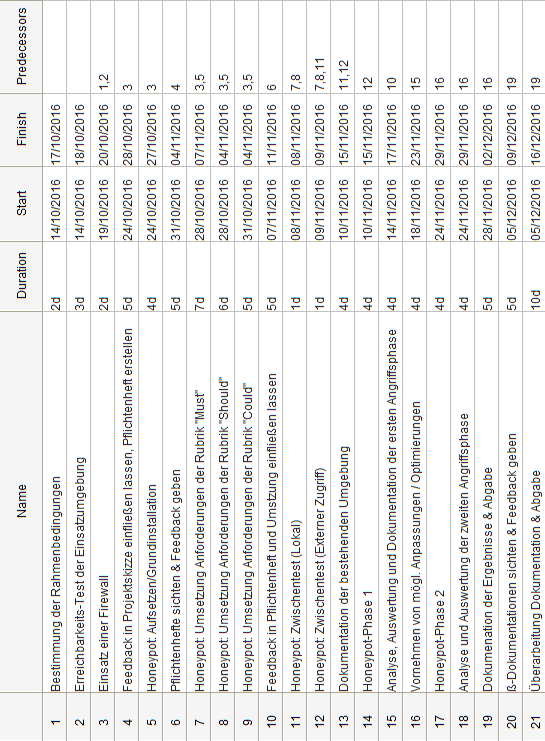
\includegraphics[scale=0.83]{img/gantt_tasks.png}
\end{center}

\newpage

\begin{center}
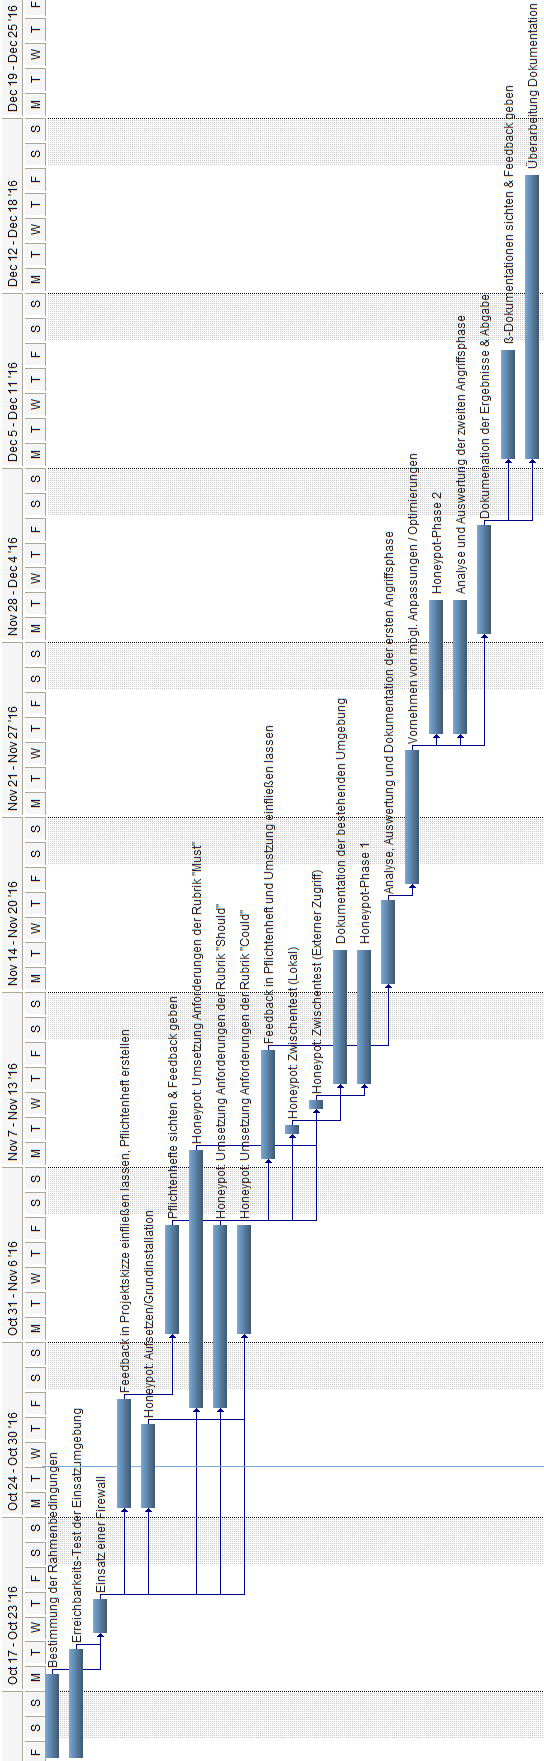
\includegraphics[scale=0.50]{img/gantt_diagram.png}
\end{center}


\section*{Selbst"andigkeitserkl"arung}
%\addcontentsline{toc}{section}{Selbst"andigkeitserkl"arung}
\thispagestyle{empty}


Ich versichere, dass ich die vorliegende Dokumentation selbständig verfasst und keine anderen als die angegebenen Quellen und Hilfsmittel benutzt habe.\\
\setlength{\parindent}{0pt}\\
Die Tabellen, Abbildungen oder Listings in dieser Arbeit sind von mir selbst erstellt worden oder mit einem entsprechenden Quellennachweis versehen.

\vspace{0.5cm}\noindent\hspace{1.5cm}

Weingarten, den 02. Dezember 2016

\vspace{1cm}\noindent\hspace{1.5cm}

Unterschrift: \noindent\hspace*{10mm}...........................\hspace*{10mm}...........................\\
\noindent\hspace*{34.5mm}Michael Stroh\hspace*{16.2mm}Daniel Schwenk


\newpage
\thispagestyle{empty}
\chapter*{ }
\thispagestyle{empty}

\end{document}
